% beyond.tex

\section{Beyond Partitioning}
\label{sec:SMPdesign:Beyond Partitioning}
\OriginallyPublished{Section}{sec:SMPdesign:Beyond Partitioning}{Retrofitted Parallelism Considered Grossly Sub-Optimal}{4\textsuperscript{th} USENIX Workshop on Hot Topics on Parallelism}{PaulEMcKenney2012HOTPARsuboptimal}

이 챕터에서는 데이터 파티셔닝이 간단한 선형적으로 확장 가능한 병렬 프로그램을
설계하는데 사용될 수 있는지 알아봤습니다.
Section~\ref{sec:SMPdesign:Data Ownership} 에서는 데이터 복사 가능성에서 힌트를
얻었는데, 이는 Section~\ref{sec:defer:Read-Copy Update (RCU)} 에서 커다란
효과를 가져올 것입니다.

파티셔닝과 복사본 사용을 적용하는 주요 목표는 선형적인 속도 향상을 얻기 위한
것으로, 달리 말하자면 CPU 나 쓰레드의 수가 늘어남에 따라 전체적으로 필요한 일의
양이 크게 늘어나지는 않음을 보장하기 위한 것입니다.
파티셔닝과 복사본 사용을 통해 해결될 수 있어서 선형적인 속도향상이 가능한
문제들은 \emph{당혹스럽게 병렬적} 입니다.
하지만 이보다 더 잘할 수는 없을까요?
\iffalse

This chapter has discussed how data partitioning can be used to design
simple linearly scalable parallel programs.
Section~\ref{sec:SMPdesign:Data Ownership} hinted at the possibilities
of data replication, which will be used to great effect in
Section~\ref{sec:defer:Read-Copy Update (RCU)}.

The main goal of applying partitioning and replication is to achieve
linear speedups, in other words, to ensure that the total amount of
work required does not increase significantly as the number of CPUs
or threads increases.
A problem that can be solved via partitioning and/or replication,
resulting in linear speedups, is \emph{embarrassingly parallel}.
But can we do better?
\fi

이 질문에 답을 하기 위해, 미궁과 미로의 해결책을 생각해 보도록 합시다.
물론, 미궁과 미로는 수천년동안 매력적인 것이었으며~\cite{WikipediaLabyrinth},
따라서 그것들이 바이오 컴퓨터~\cite{AndrewAdamatzky2011SlimeMold},
GPGPU~\cite{ChristerEricson2008GPUMaze}, 심지어는 분리된
하드웨어~\cite{MIT:TRMag:MemristorMazes} 등의 컴퓨터들을 사용해서 만들어지고
해결되었음은 별로 놀라운 일도 아닙니다.
미로의 병렬적 해결책은 대학 수업에서의 과제
프로젝트~\cite{ETHZurich:FS2011maze,UMD:CMSC433maze} 로도 사용되었고, 병렬
프로그래밍 프레임웍의 이점을 보이기 위한 매개물~\cite{RonFosner2010maze} 로도
사용되었습니다.
\iffalse

To answer this question, let us examine the solution of
labyrinths and mazes.
Of course, labyrinths and mazes have been objects of fascination for
millennia~\cite{WikipediaLabyrinth},
so it should come as no surprise that they are generated and solved
using computers, including biological
computers~\cite{AndrewAdamatzky2011SlimeMold},
GPGPUs~\cite{ChristerEricson2008GPUMaze}, and even
discrete hardware~\cite{MIT:TRMag:MemristorMazes}.
Parallel solution of mazes is sometimes used as a class project in
universities~\cite{ETHZurich:FS2011maze,UMD:CMSC433maze} and
as a vehicle to demonstrate the benefits of parallel-programming
frameworks~\cite{RonFosner2010maze}.
\fi

흔한 조언은 병렬 일거리-대기열 알고리즘(PWQ: Parallel work-queue
algorithm)~\cite{ETHZurich:FS2011maze,RonFosner2010maze} 을 사용하라는
것입니다.
이 섹션은 무작위적으로 생성된 정사각형의 미로를 해결하는 모든 경우에 대해
순차적 알고리즘 (SEQ) 과 대안적인 병렬 알고리즘에 대해 PWQ 를 비교하는 것으로
이 조언을 평가해 보겠습니다.
Section~\ref{sec:SMPdesign:Work-Queue Parallel Maze Solver} 에서는 PWQ 를
이야기 하고,
Section~\ref{sec:SMPdesign:Alternative Parallel Maze Solver} 에서 대안적인 병렬
알고리즘을 설명하며,
Section~\ref{sec:SMPdesign:Performance Comparison I} 에서는 그것의 문제 있는
성능에 대해 이야기 한 후,
Section~\ref{sec:SMPdesign:Alternative Sequential Maze Solver} 에서 앞의 대안적
병렬 알고리즘으로부터 향상된 순차적 알고리즘을 소개하며,
Section~\ref{sec:SMPdesign:Performance Comparison II} 에서 성능을 비교해 보고,
마지막으로
Section~\ref{sec:SMPdesign:Future Directions and Conclusions} 에서 미래의
방향을 알아보고 결론을 내려봅니다.
\iffalse

Common advice is to use a parallel work-queue algorithm
(PWQ)~\cite{ETHZurich:FS2011maze,RonFosner2010maze}.
This section evaluates this advice by comparing PWQ
against a sequential algorithm (SEQ) and also against
an alternative parallel algorithm, in all cases solving randomly generated
square mazes.
Section~\ref{sec:SMPdesign:Work-Queue Parallel Maze Solver} discusses PWQ,
Section~\ref{sec:SMPdesign:Alternative Parallel Maze Solver} discusses an alternative
parallel algorithm,
Section~\ref{sec:SMPdesign:Performance Comparison I} analyzes its anomalous performance,
Section~\ref{sec:SMPdesign:Alternative Sequential Maze Solver} derives an improved
sequential algorithm from the alternative parallel algorithm,
Section~\ref{sec:SMPdesign:Performance Comparison II} makes further performance
comparisons,
and finally
Section~\ref{sec:SMPdesign:Future Directions and Conclusions}
presents future directions and concluding remarks.
\fi

\subsection{Work-Queue Parallel Maze Solver}
\label{sec:SMPdesign:Work-Queue Parallel Maze Solver}

\begin{listing}[tbp]
{ \scriptsize
\begin{verbbox}
  1 int maze_solve(maze *mp, cell sc, cell ec)
  2 {
  3   cell c = sc;
  4   cell n;
  5   int vi = 0;
  6 
  7   maze_try_visit_cell(mp, c, c, &n, 1);
  8   for (;;) {
  9     while (!maze_find_any_next_cell(mp, c, &n)) {
 10       if (++vi >= mp->vi)
 11         return 0;
 12       c = mp->visited[vi].c;
 13     }
 14     do {
 15       if (n == ec) {
 16         return 1;
 17       }
 18       c = n;
 19     } while (maze_find_any_next_cell(mp, c, &n));
 20     c = mp->visited[vi].c;
 21   }
 22 }
\end{verbbox}
}
\centering
\theverbbox
\caption{SEQ Pseudocode}
\label{lst:SMPdesign:SEQ Pseudocode}
\end{listing}

PWQ 는 Listing~\ref{lst:SMPdesign:SEQ Pseudocode}(\co{maze_seq.c}) 에 있는 SEQ
에 기반합니다.
미로는 셀들의 2D 배열과 \co{->visited} 로 이름 붙여진 선형적 배열 기반 일거리
대기열로 나타내어집니다.

Line~7 에서 첫번째 셀에 들어가고, line~8-21 에 있는 루프의 매 반복에서 하나의
셀에 의해 향해지는 통로를 횡단합니다.
Line9-13 의 루프에서는 \co{->visited[]} 배열을 방문되지 않은 이웃을 가지고
방문된 셀을 위해 스캔하고, line~14-19 의 루프에서는 그 이웃을 통해 향해지는
작은 미로를 횡단합니다.
Line~20 에서는 밖의 루프에 의해 통과될 다음 경로를 위해 초기화를 합니다.
\iffalse

PWQ is based on SEQ, which is shown in
Listing~\ref{lst:SMPdesign:SEQ Pseudocode}
(\path{maze_seq.c}).
The maze is represented by a 2D array of cells and
a linear-array-based work queue named \co{->visited}.

Line~7 visits the initial cell, and each iteration of the loop spanning
lines~8-21 traverses passages headed by one cell.
The loop spanning lines~9-13 scans the \co{->visited[]} array for a
visited cell with an unvisited neighbor, and the loop spanning
lines~14-19 traverses one fork of the submaze headed by that neighbor.
Line~20 initializes for the next pass through the outer loop.
\fi

\begin{listing}[tbp]
{ \scriptsize
\begin{verbbox}
  1 int maze_try_visit_cell(struct maze *mp, cell c, cell t,
  2                         cell *n, int d)
  3 {
  4   if (!maze_cells_connected(mp, c, t) ||
  5       (*celladdr(mp, t) & VISITED))
  6     return 0;
  7   *n = t;
  8   mp->visited[mp->vi] = t;
  9   mp->vi++;
 10   *celladdr(mp, t) |= VISITED | d;
 11   return 1;
 12 }
 13 
 14 int maze_find_any_next_cell(struct maze *mp, cell c,
 15                             cell *n)
 16 {
 17   int d = (*celladdr(mp, c) & DISTANCE) + 1;
 18 
 19   if (maze_try_visit_cell(mp, c, prevcol(c), n, d))
 20     return 1;
 21   if (maze_try_visit_cell(mp, c, nextcol(c), n, d))
 22     return 1;
 23   if (maze_try_visit_cell(mp, c, prevrow(c), n, d))
 24     return 1;
 25   if (maze_try_visit_cell(mp, c, nextrow(c), n, d))
 26     return 1;
 27   return 0;
 28 }
\end{verbbox}
}
\centering
\theverbbox
\caption{SEQ Helper Pseudocode}
\label{lst:SMPdesign:SEQ Helper Pseudocode}
\end{listing}

\co{maze_try_visit_cell()} 의 슈도코드가
Listing~\ref{lst:SMPdesign:SEQ Helper Pseudocode}
(\co{maze.c}) 의 line~1-12 에 나타나
있습니다.
Line~4 에서셀 \co{c} 와 \co{n} 이 근처에 있고 연결되어 있는지 체크해 보고,
line~5 에서는 셀 \co{n} 이 아직 방문되지 않았는지 확인해 봅니다.
\co{celladdr()} 함수는 지목된 셀의 주소를 리턴합니다.
두 체크 중 하나라도 실패하면, line~6 에서 실패했음을 리턴합니다.
Line~7 에서는 다음 셀을 알리고, line~8 에서 이 셀을 \co{->visited[]} 배열의
다음 슬롯에 기록해 두고, line~9 에서 이 슬롯이 이제 채워졌음을 알리며, line~10
에서 이 셀을 방문되었음으로 마크하고 미로의 시작점으로부터의 거리를 기록해
둡니다.
Line~11 은 이제 성공했음을 리턴합니다.

\co{maze_find_any_next_cell()} 의 슈도코드가
Listing~\ref{lst:SMPdesign:SEQ Helper Pseudocode}
(\co{maze.c}) 의 line~14-28 에 있습니다.
Line~17 에서는 현재 셀의 거리 더하기 1을 얻어오고, 라인~19, 21, 23, 25 에서는
각 방향의 해당 셀들을 체크하고, ine~20, 22, 24, 26 에서는 연관된 셀이 다음 셀
후보라면 \co{true} 를 리턴합니다.
\co{prevcol()}, \co{nextcol()}, \co{prevrow()}, 그리고 \co{nextrow()} 는 각각
배열 인덱스 변환 작업을 수행합니다.
어떤 셀도 후보가 아니라면, line~27 에서 \co{false} 를 리턴합니다.
\iffalse

The pseudocode for \co{maze_try_visit_cell()} is shown on lines~1-12
of Listing~\ref{lst:SMPdesign:SEQ Helper Pseudocode}
(\path{maze.c}).
Line~4 checks to see if cells \co{c} and \co{n} are adjacent and connected,
while line~5 checks to see if cell \co{n} has not yet been visited.
The \co{celladdr()} function returns the address of the specified cell.
If either check fails, line~6 returns failure.
Line~7 indicates the next cell, line~8 records this cell in the next
slot of the \co{->visited[]} array, line~9 indicates that this slot
is now full, and line~10 marks this cell as visited and also records
the distance from the maze start.  Line~11 then returns success.

The pseudocode for \co{maze_find_any_next_cell()} is shown on lines~14-28
of Listing~\ref{lst:SMPdesign:SEQ Helper Pseudocode}
(\path{maze.c}).
Line~17 picks up the current cell's distance plus 1,
while lines~19, 21, 23, and~25
check the cell in each direction, and lines~20, 22, 24, and~26
return true if the corresponding cell is a candidate next cell.
The \co{prevcol()}, \co{nextcol()}, \co{prevrow()}, and \co{nextrow()}
each do the specified array-index-conversion operation.
If none of the cells is a candidate, line~27 returns false.
\fi

\begin{figure}[tb]
\centering
\resizebox{1.2in}{!}{\includegraphics{SMPdesign/MazeNumberPath}}
\caption{Cell-Number Solution Tracking}
\label{fig:SMPdesign:Cell-Number Solution Tracking}
\end{figure}

해당 경로는 Figure~\ref{fig:SMPdesign:Cell-Number Solution Tracking} 에
보여지는 것처럼, 미로에 시작점으로부터의 셀들의 수를 세는 것으로 기록되는데,
시작 셀은 좌상단에 위치해 있고 끝의 셀은 우하단에 위치해 있습니다.
끝 셀로부터 시작해서 연속적으로 줄어드는 셀 숫자들을 따라가는 것으로 해결
경로를 따라 횡단할 수 있습니다.
\iffalse

The path is recorded in the maze by counting the number of cells from
the starting point, as shown in
Figure~\ref{fig:SMPdesign:Cell-Number Solution Tracking},
where the starting cell is in the upper left and the ending cell is
in the lower right.
Starting at the ending cell and following
consecutively decreasing cell numbers traverses the solution.
\fi

\begin{figure}[tb]
\centering
\resizebox{2.2in}{!}{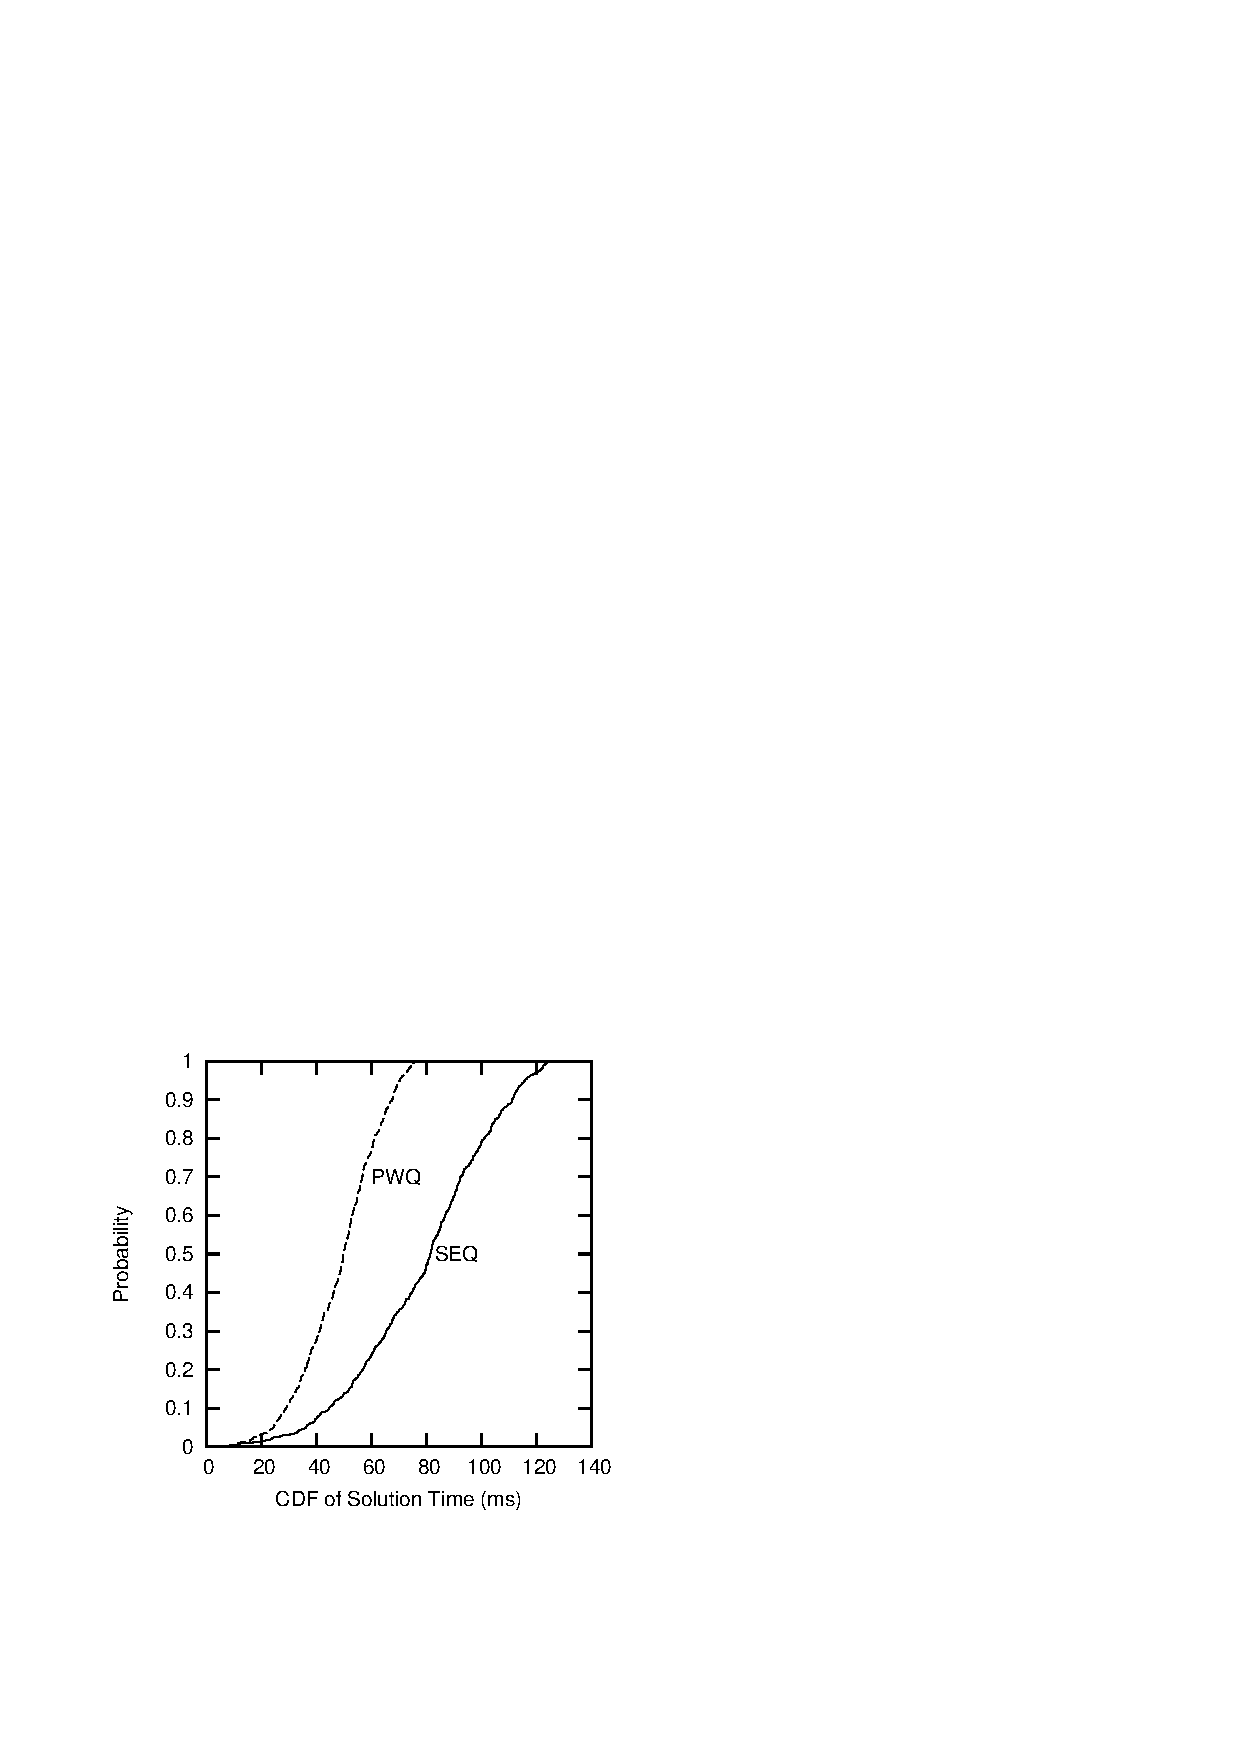
\includegraphics{SMPdesign/500-ms_seq_fg-cdf}}
\caption{CDF of Solution Times For SEQ and PWQ}
\label{fig:SMPdesign:CDF of Solution Times For SEQ and PWQ}
\end{figure}

병렬 작업 대기열 처리자 (work-queue solver) 는
Listing~\ref{lst:SMPdesign:SEQ Pseudocode} 와
~\ref{lst:SMPdesign:SEQ Helper Pseudocode} 에 보여진 알고리즘의 직선적인
병렬화입니다.
Listing~\ref{lst:SMPdesign:SEQ Pseudocode} 의 line~10 은 fetch-and-add 를
사용해야만 하고 지역 변수인 \co{vi} 는 여러 쓰레드들 사이에 공유되어야만
합니다.
Listing~\ref{lst:SMPdesign:SEQ Helper Pseudocode} 의 Line~5 와~10 은 CAS 루프로
구성되어야만 하는데, 이 때 CAS 의 실패는 미로 루프를 의미하게 됩니다.
이 그림의 Line~8-9 는 셀들을 \co{->visited[]} 배열에 동시적으로 기록하려
시도하는 것을 처리하기 위해 fetch-and-add 를 사용해야만 합니다.
\iffalse

The parallel work-queue solver is a straightforward parallelization
of the algorithm shown in
Listings~\ref{lst:SMPdesign:SEQ Pseudocode} and~\ref{lst:SMPdesign:SEQ Helper Pseudocode}.
Line~10 of Listing~\ref{lst:SMPdesign:SEQ Pseudocode} must use fetch-and-add,
and the local variable \co{vi} must be shared among the various threads.
Lines~5 and~10 of Listing~\ref{lst:SMPdesign:SEQ Helper Pseudocode} must be
combined into a CAS loop, with CAS failure indicating a loop in the
maze.
Lines~8-9 of this listing must use fetch-and-add to arbitrate concurrent
attempts to record cells in the \co{->visited[]} array.
\fi

이 접근법은 Figure~\ref{fig:SMPdesign:CDF of Solution Times For SEQ and PWQ}
에서 볼 수 있듯이 2.53GHz 의 속도로 동작하는 dual-CPU
Lenovo\textsuperscript\texttrademark W500 에서 상당한 속도 향상을 보여주는데,
두 알고리즘의 해결책을 얻는데 걸리는 시간의 누적 분포 함수들 (CDF) 을 500 개의
다른 500행 500열의 정사각으로 무작위적으로 만들어진 미로들에 대해
측정되었습니다.
이 CDF 들을 x 축에 투영해서 만들어지는 실질적인 겹쳐진 모습은
Section~\ref{sec:SMPdesign:Performance Comparison I} 에서 다루어질 것입니다.

상당히 흥미롭게도, 순차적인 해결책의 경로 탐색은 병렬 알고리즘에서도 바뀌지
않았습니다.
하지만, 이는 병렬 알고리즘의 상당한 약점을 드러냈습니다:
어떤 주어진 시간 동안 최대 하나의 쓰레드만이 해결책 경로로의 진행을 만들 수
있습니다.
이 약점은 다음 섹션에서 다루어집니다.
\iffalse


This approach does provide significant speedups on a dual-CPU
Lenovo\mytexttrademark\ W500
running at 2.53\,GHz, as shown in
Figure~\ref{fig:SMPdesign:CDF of Solution Times For SEQ and PWQ},
which shows the cumulative distribution functions (CDFs) for the solution
times of the two algorithms, based on the solution of 500 different square
500-by-500 randomly generated mazes.
The substantial overlap
of the projection of the CDFs onto the x-axis will be addressed in
Section~\ref{sec:SMPdesign:Performance Comparison I}.

Interestingly enough, the sequential solution-path tracking works unchanged
for the parallel algorithm.
However, this uncovers a significant weakness in the parallel algorithm:
At most one thread may be making progress along the solution path at
any given time.
This weakness is addressed in the next section.
\fi

\subsection{Alternative Parallel Maze Solver}
\label{sec:SMPdesign:Alternative Parallel Maze Solver}

유용한 미로 풀기 방법들은 종종 양 끝에서 시작할 것을 주장했고, 이런 조언은
자동화된 미로 해법~\cite{UMD:CMSC433maze} 의 맥락에서 최근들어 더
반복되었습니다.
이 조언은 파티셔닝과 같은 것으로, 파티셔닝은 병렬 프로그래밍의 맥락에서
운영체제 커널에 대해서도~\cite{Beck85,Inman85} 어플리케이션에
대해서도~\cite{DavidAPatterson2010TroubleMulticore} 강력한 병렬화 전략이
되어왔습니다.
이 섹션에서는 이 전략을 적용해 보는데, 해결책 경로의 양 끝단에서 시작하는
두개의 자식 쓰레드를 사용하고, 성능과 확장성에 대해 짧게 결과를 알아봅니다.
\iffalse

Youthful maze solvers are often urged to start at both ends, and
this advice has been repeated more recently in the context of automated
maze solving~\cite{UMD:CMSC433maze}.
This advice amounts to partitioning, which has been a powerful
parallelization strategy
in the context of parallel programming for both operating-system
kernels~\cite{Beck85,Inman85} and
applications~\cite{DavidAPatterson2010TroubleMulticore}.
This section applies this strategy, using two child threads that start
at opposite ends of the solution path, and takes a brief look at the
performance and scalability consequences.
\fi

\begin{listing}[tbp]
{ \scriptsize
\begin{verbbox}
  1 int maze_solve_child(maze *mp, cell *visited, cell sc)
  2 {
  3   cell c;
  4   cell n;
  5   int vi = 0;
  6 
  7   myvisited = visited; myvi = &vi;
  8   c = visited[vi];
  9   do {
 10     while (!maze_find_any_next_cell(mp, c, &n)) {
 11       if (visited[++vi].row < 0)
 12         return 0;
 13       if (ACCESS_ONCE(mp->done))
 14         return 1;
 15       c = visited[vi];
 16     }
 17     do {
 18       if (ACCESS_ONCE(mp->done))
 19         return 1;
 20       c = n;
 21     } while (maze_find_any_next_cell(mp, c, &n));
 22     c = visited[vi];
 23   } while (!ACCESS_ONCE(mp->done));
 24   return 1;
 25 }
\end{verbbox}
}
\centering
\theverbbox
\caption{Partitioned Parallel Solver Pseudocode}
\label{lst:SMPdesign:Partitioned Parallel Solver Pseudocode}
\end{listing}

Listing~\ref{lst:SMPdesign:Partitioned Parallel Solver Pseudocode}
(\co{maze_part.c}) 에 보여진 파티션을 사용한 병렬 알고리즘 (PART) 는 SEQ 와
비슷하지만 몇가지 중요한 차이점이 있습니다.
첫번째로, 각 자식 쓰레드는 자신의 \co{visited} 배열을 가지고 있는데, line~1
에서 보듯이 부모로부터 전달받은 것으로, 모두 [-1,-1] 로 초기화 되어 있어야만
합니다.
Line~7 에서는 이 배열로의 포인터를 per-thread 변수 \co{myvisited} 에 저장해서
도우미 함수들로부터의 접근을 가능하게 하고, 비슷하게 지역적으로 방문한 곳의
인덱스로의 포인터를 저장합니다.
두번째로, 부모는 각 자식의 입장에서 첫번째 셀을 방문하는데, 이는 자식들이
line~8 에서 얻어옵니다.
세번째로, 미로는 한 자식이 다른 자식에 의해 방문되었던 셀을 발견하면 그 즉시
풀이됩니다.
\co{maze_try_visit_cell()} 이 이를 발견하게 되면, 이 함수는 해당 미로 구조체의
\co{->done} 필드에 값을 넣습니다.
넷째로, 따라서 각 자식은 line~13, 18, 23 에 보여진 것처럼 주기적으로
\co{->done} 필드를 체크해야만 합니다.
\co{ACCESS_ONCE()} 기능은 다음의 연속적인 로드들을 합치거나 값을 다시 읽어올
수도 있는 어떤 컴파일러 최적화도 무력화 되도록 해야만 합니다.
이를 위해선 C++1x volatile relaxed load 로도
충분합니다~\cite{PeteBecker2011N3242}.
마지막으로, \co{maze_find_and_next_cell()} 함수는 한 셀을 방문된 것으로
마크하기 위해 compare-and-swap 을 사용해야만 합니다만, 쓰레드 생성과 합치기에
의해 만들어지는 순서 이후에 어떤 순서 제약도 필요시 되지 않습니다.
\iffalse

The partitioned parallel algorithm (PART), shown in
Listing~\ref{lst:SMPdesign:Partitioned Parallel Solver Pseudocode}
(\path{maze_part.c}),
is similar to SEQ, but has a few important differences.
First, each child thread has its own \co{visited} array, passed in by
the parent as shown on line~1,
which must be initialized to all [$-1$, $-1$].
Line~7 stores a pointer to this array into the per-thread variable
\co{myvisited} to allow access by helper functions, and similarly stores
a pointer to the local visit index.
Second, the parent visits the first cell on each child's behalf,
which the child retrieves on line~8.
Third, the maze is solved as soon as one child locates a cell that has
been visited by the other child.
When \co{maze_try_visit_cell()} detects this,
it sets a \co{->done} field in the maze structure.
Fourth, each child must therefore periodically check the \co{->done}
field, as shown on lines~13, 18, and~23.
The \co{ACCESS_ONCE()} primitive must disable any compiler
optimizations that might combine consecutive loads or that
might reload the value.
A C++1x volatile relaxed load suffices~\cite{PeteBecker2011N3242}.
Finally, the \co{maze_find_any_next_cell()} function must use
compare-and-swap to mark a cell as visited, however
no constraints on ordering are required beyond those provided by
thread creation and join.
\fi

\begin{listing}[tbp]
{ \scriptsize
\begin{verbbox}
  1 int maze_try_visit_cell(struct maze *mp, int c, int t,
  2       int *n, int d)
  3 {
  4   cell_t t;
  5   cell_t *tp;
  6   int vi;
  7 
  8   if (!maze_cells_connected(mp, c, t))
  9     return 0;
 10   tp = celladdr(mp, t);
 11   do {
 12     t = ACCESS_ONCE(*tp);
 13     if (t & VISITED) {
 14       if ((t & TID) != mytid)
 15         mp->done = 1;
 16       return 0;
 17     }
 18   } while (!CAS(tp, t, t | VISITED | myid | d));
 19   *n = t;
 20   vi = (*myvi)++;
 21   myvisited[vi] = t;
 22   return 1;
 23 }
\end{verbbox}
}
\centering
\theverbbox
\caption{Partitioned Parallel Helper Pseudocode}
\label{lst:SMPdesign:Partitioned Parallel Helper Pseudocode}
\end{listing}

\co{maze_find_any_next_cell()} 의 슈도코드는
Listing~\ref{lst:SMPdesign:SEQ Helper Pseudocode} 에 보여진 것과 동일합니다만,
\co{maze_try_visit_cell()} 의 슈도코드는 좀 다른데,
Listing~\ref{lst:SMPdesign:Partitioned Parallel Helper Pseudocode} 에 보여져
있습니다.
Line~8-9 는 해당 셀들이 연결되어 있는지 체크하고, 그렇지 않다면 failure 를
리턴합니다.
Line~11-18 의 루프에서는 새 셀을 방문된 것으로 마크합니다.
Line~13 은 해당 셀이 이미 방문된 적 있는지 체크하고, 이 경우엔 line~16 에서
failure 를 리턴합니다만, line~14 에서 다른 쓰레드와 마주친 것인지 체크한
이후로, 마주친 경우라면 line~15 에서 해법이 찾아졌음을 알립니다.
Line~19 에서는 새 셀에 업데이트를 하고, line~20 과 21 에서 이 쓰레드의 방문된
곳 배열을 업데이트 하며, line~22 에서 success 를 리턴합니다.
\iffalse

The pseudocode for \co{maze_find_any_next_cell()} is identical to that shown in
Listing~\ref{lst:SMPdesign:SEQ Helper Pseudocode},
but the pseudocode for \co{maze_try_visit_cell()} differs, and
is shown in
Listing~\ref{lst:SMPdesign:Partitioned Parallel Helper Pseudocode}.
Lines~8-9 check to see if the cells are connected, returning failure
if not.
The loop spanning lines~11-18 attempts to mark the new cell visited.
Line~13 checks to see if it has already been visited, in which case
line~16 returns failure, but only after line~14 checks to see if
we have encountered the other thread, in which case line~15 indicates
that the solution has been located.
Line~19 updates to the new cell, lines~20 and~21 update this thread's visited
array, and line~22 returns success.
\fi

\begin{figure}[tb]
\centering
\resizebox{2.2in}{!}{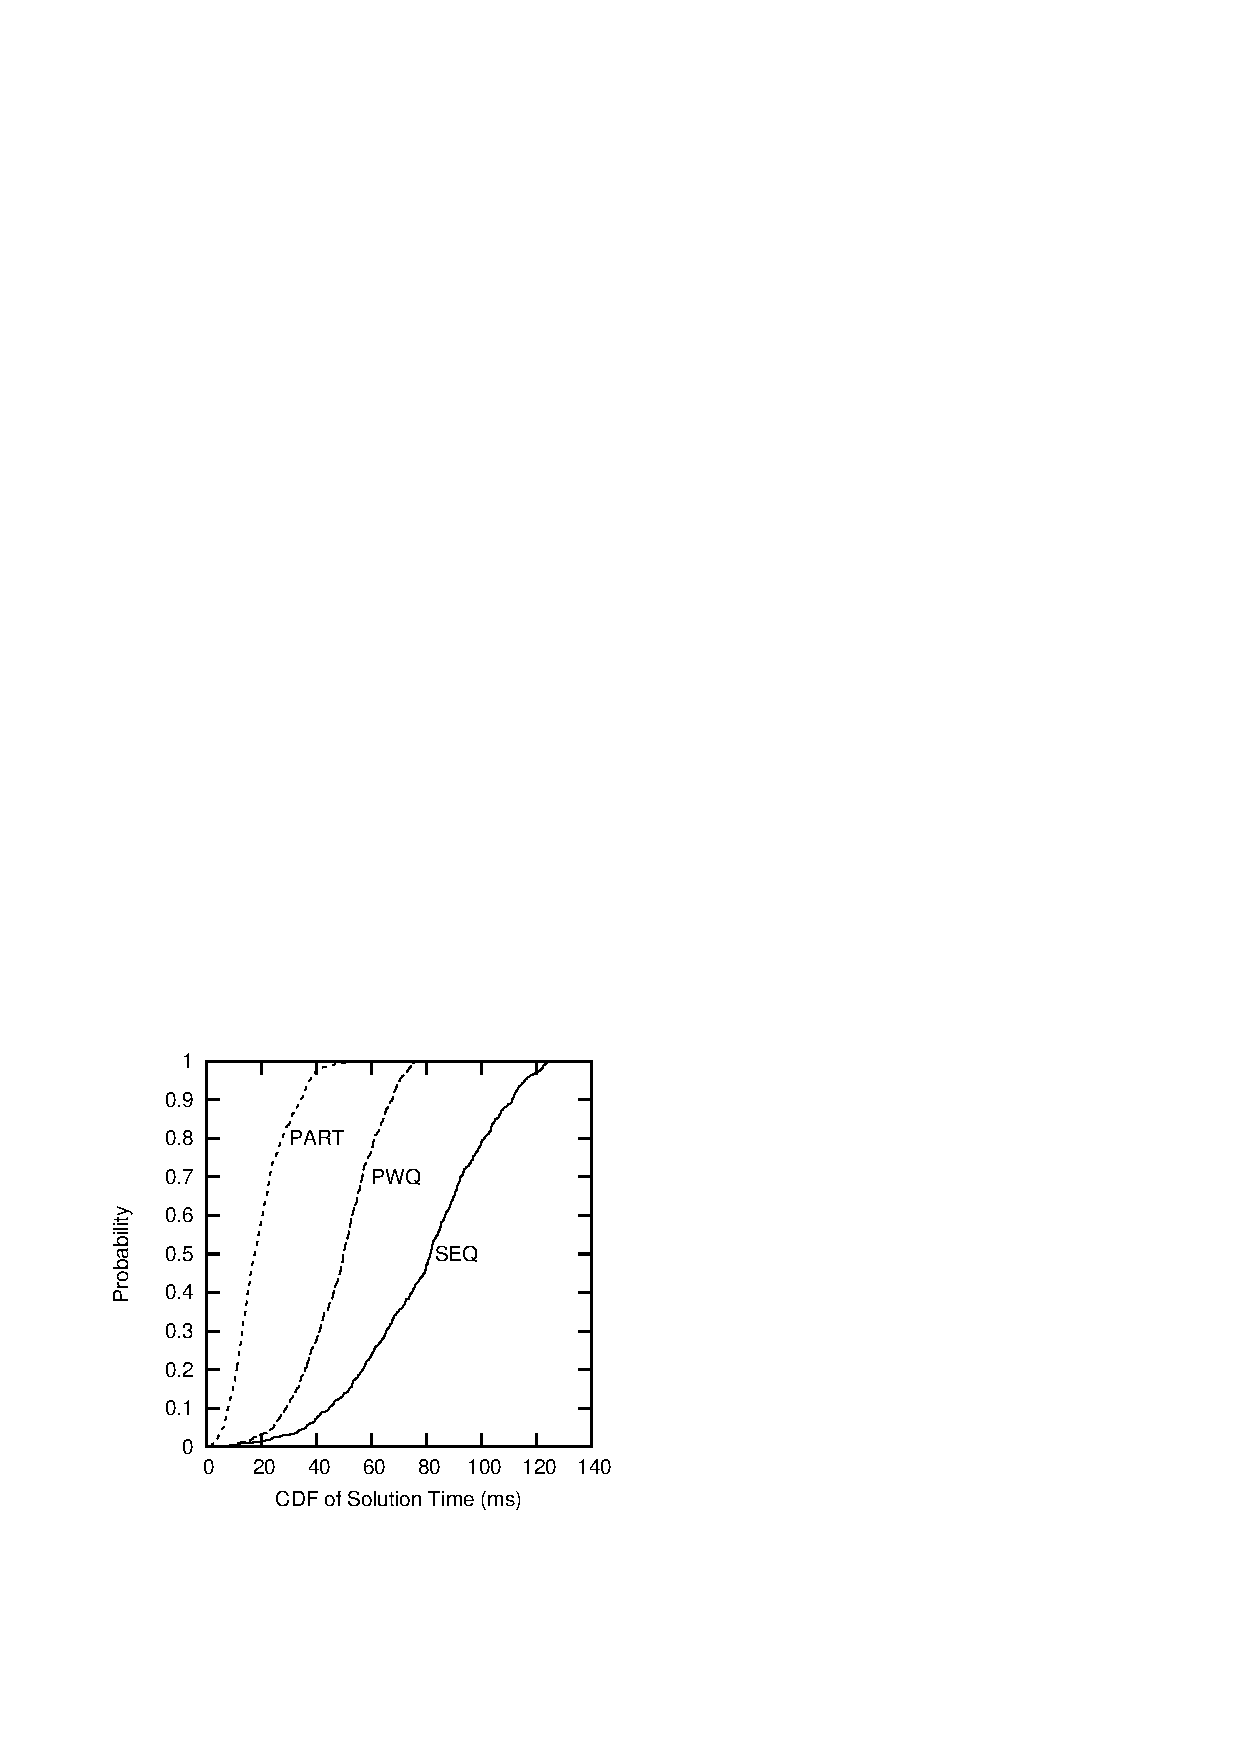
\includegraphics{SMPdesign/500-ms_seq_fg_part-cdf}}
\caption{CDF of Solution Times For SEQ, PWQ, and PART}
\label{fig:SMPdesign:CDF of Solution Times For SEQ, PWQ, and PART}
\end{figure}

성능 테스트는
Figure~\ref{fig:SMPdesign:CDF of Solution Times For SEQ, PWQ, and PART} 에
보여진 것과 같이 심각한 변칙적 결과를 보였습니다.
PART 의 평균 해법 탐색 시간 (17 밀리세컨드) 은 SEQ 의 그것 (79 밀리세컨드) 보다
두개의 쓰레드만 사용함에도 네배 넘게 빨랐습니다.
다음 섹션에서 이 결과를 분석해 봅니다.
\iffalse

Performance testing revealed a surprising anomaly, shown in
Figure~\ref{fig:SMPdesign:CDF of Solution Times For SEQ, PWQ, and PART}.
The median solution time for PART (17 milliseconds)
is more than four times faster than that of SEQ (79 milliseconds),
despite running on only two threads.
The next section analyzes this anomaly.
\fi

\subsection{Performance Comparison I}
\label{sec:SMPdesign:Performance Comparison I}

\begin{figure}[tb]
\centering
\resizebox{2.2in}{!}{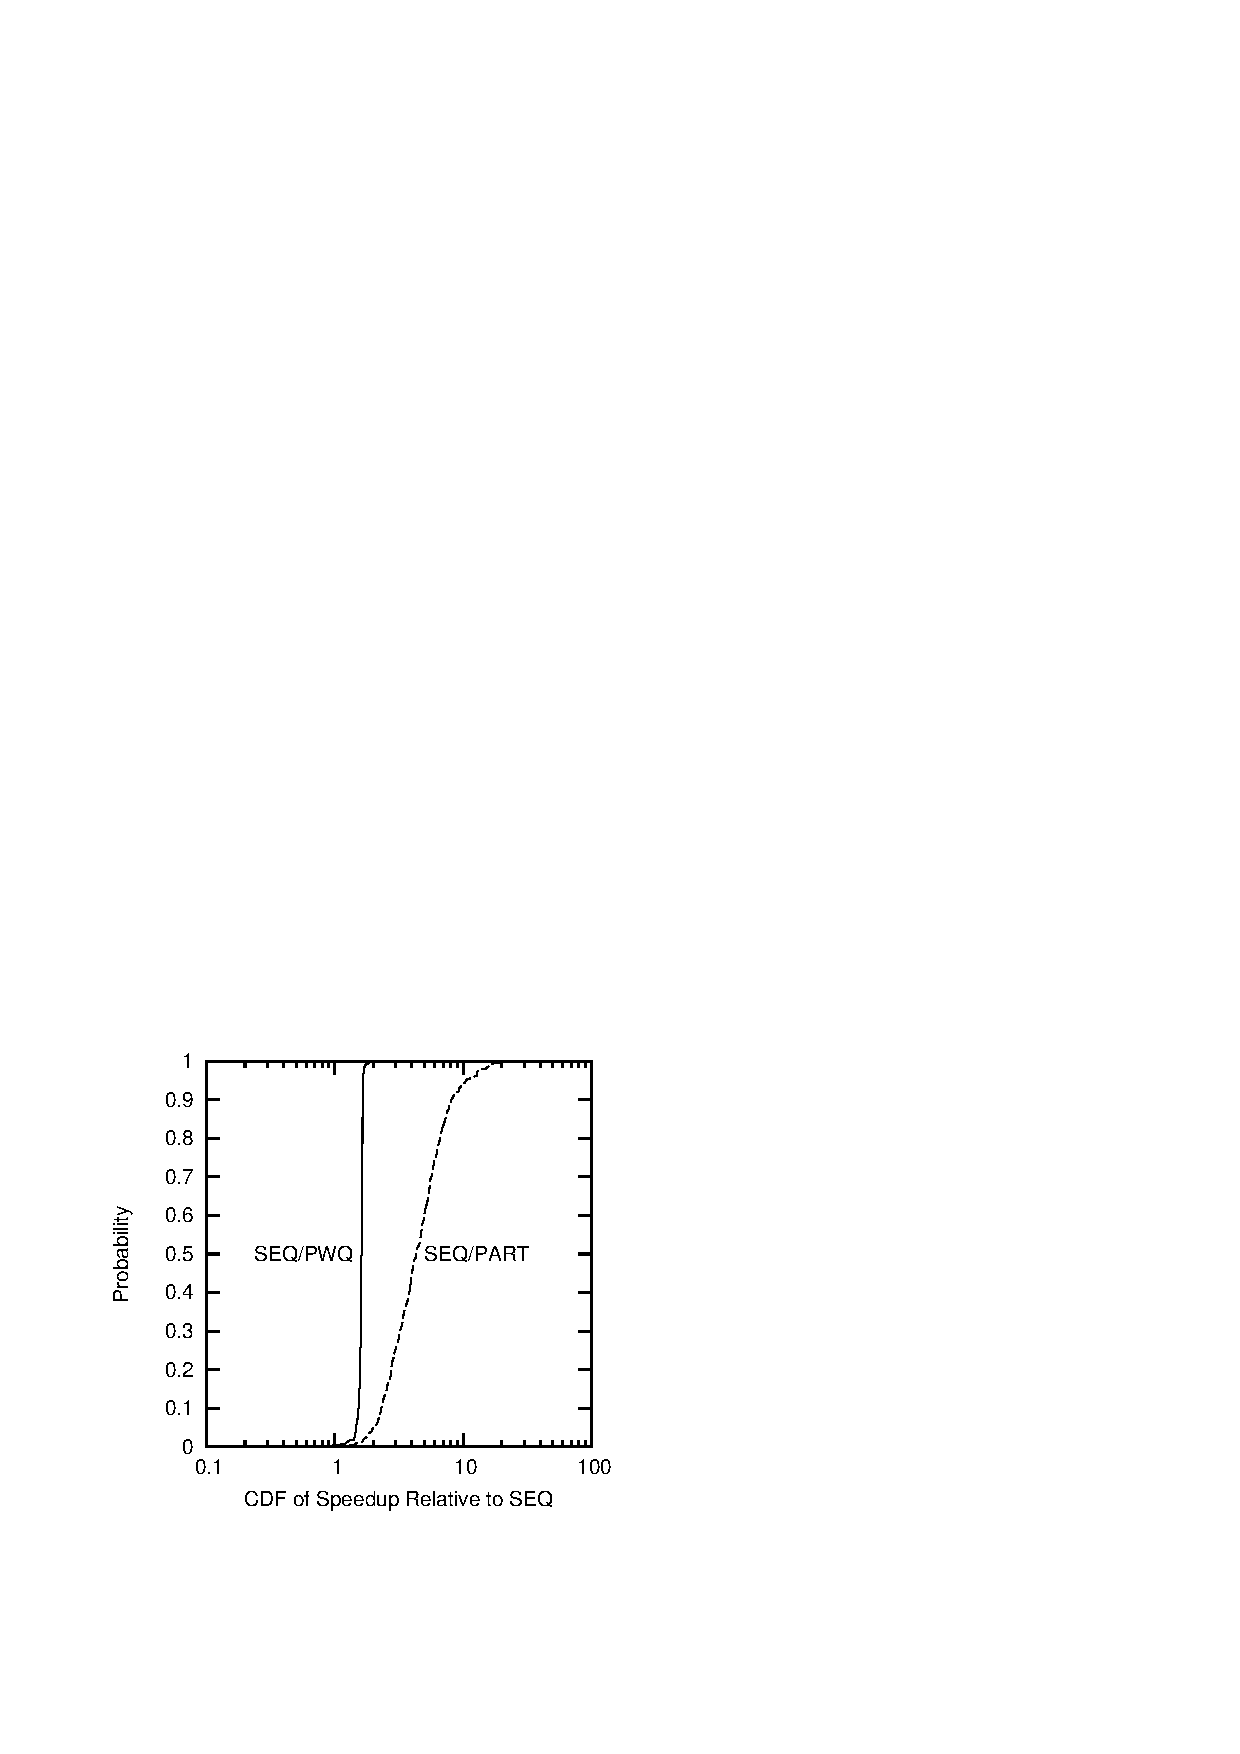
\includegraphics{SMPdesign/500-ms_seqVfg_part-cdf}}
\caption{CDF of SEQ/PWQ and SEQ/PART Solution-Time Ratios}
\label{fig:SMPdesign:CDF of SEQ/PWQ and SEQ/PART Solution-Time Ratios}
\end{figure}

이례적 성능 결과에 대한 첫번째 대응은 버그 유무를 체크하는 것입니다.
이 알고리즘들은 모두 실제로 올바른 해결책을 찾아내고 있습니다만,
Figure~\ref{fig:SMPdesign:CDF of Solution Times For SEQ, PWQ, and PART} 에
나타난 CDF 그림은 독립적인 데이터를 가정하고 있습니다.
이건 올바른 경우가 아닙니다:  이 성능 테스트들은 무작위적으로 미로를 생성하고,
그 미로에 대해 모든 알고리즘들을 돌려보고 있습니다.
따라서 각각의 생성된 미로에 대해 해결책을 찾는데 걸린 시간의 비율의 CDF 를
그려보는게 좀 더 말이 될텐데,
Figure~\ref{fig:SMPdesign:CDF of SEQ/PWQ and SEQ/PART Solution-Time Ratios} 에
그 그림이 그려져 있으며, 여기선 CDF 들의 중복이 훨씬 줄어들었습니다.
쓰레드 두개로 이루어진 40배의 성능 향상은 설명이 필요합니다.
무엇보다, 이것은 단지 파티션으로 쪼갤 수 있음이 쓰레드를 추가하는 것으로 인해
전체 연산 비용의 증가로 이어지지 않음을 의미하는 당혹스러울 정도의 병렬성도
아닙니다.
그 대신, 이것은 \emph{굴욕적인 병렬성} 입니다: 쓰레드를 추가하는 것이 전체 연산
비용을 상당히 줄여줘서 커다란 알고리즘적인 선형적인 성능향상을 초월하는 결과를
이끌어낸 것입니다. 
\iffalse

The first reaction to a performance anomaly is to check for bugs.
Although the algorithms were in fact finding valid solutions, the
plot of CDFs in
Figure~\ref{fig:SMPdesign:CDF of Solution Times For SEQ, PWQ, and PART}
assumes independent data points.
This is not the case:  The performance tests randomly generate a maze,
and then run all solvers on that maze.
It therefore makes sense to plot the CDF of the ratios of
solution times for each generated maze,
as shown in
Figure~\ref{fig:SMPdesign:CDF of SEQ/PWQ and SEQ/PART Solution-Time Ratios},
greatly reducing the CDFs' overlap.
This plot reveals that for some mazes, PART
is more than \emph{forty} times faster than SEQ.
In contrast, PWQ is never more than about
two times faster than SEQ.
A forty-times speedup on two threads demands explanation.
After all, this is not merely embarrassingly parallel, where partitionability
means that adding threads does not increase the overall computational cost.
It is instead \emph{humiliatingly parallel}: Adding threads
significantly reduces the overall computational cost, resulting in
large algorithmic superlinear speedups.
\fi

\begin{figure}[tb]
\centering
\resizebox{1.4in}{!}{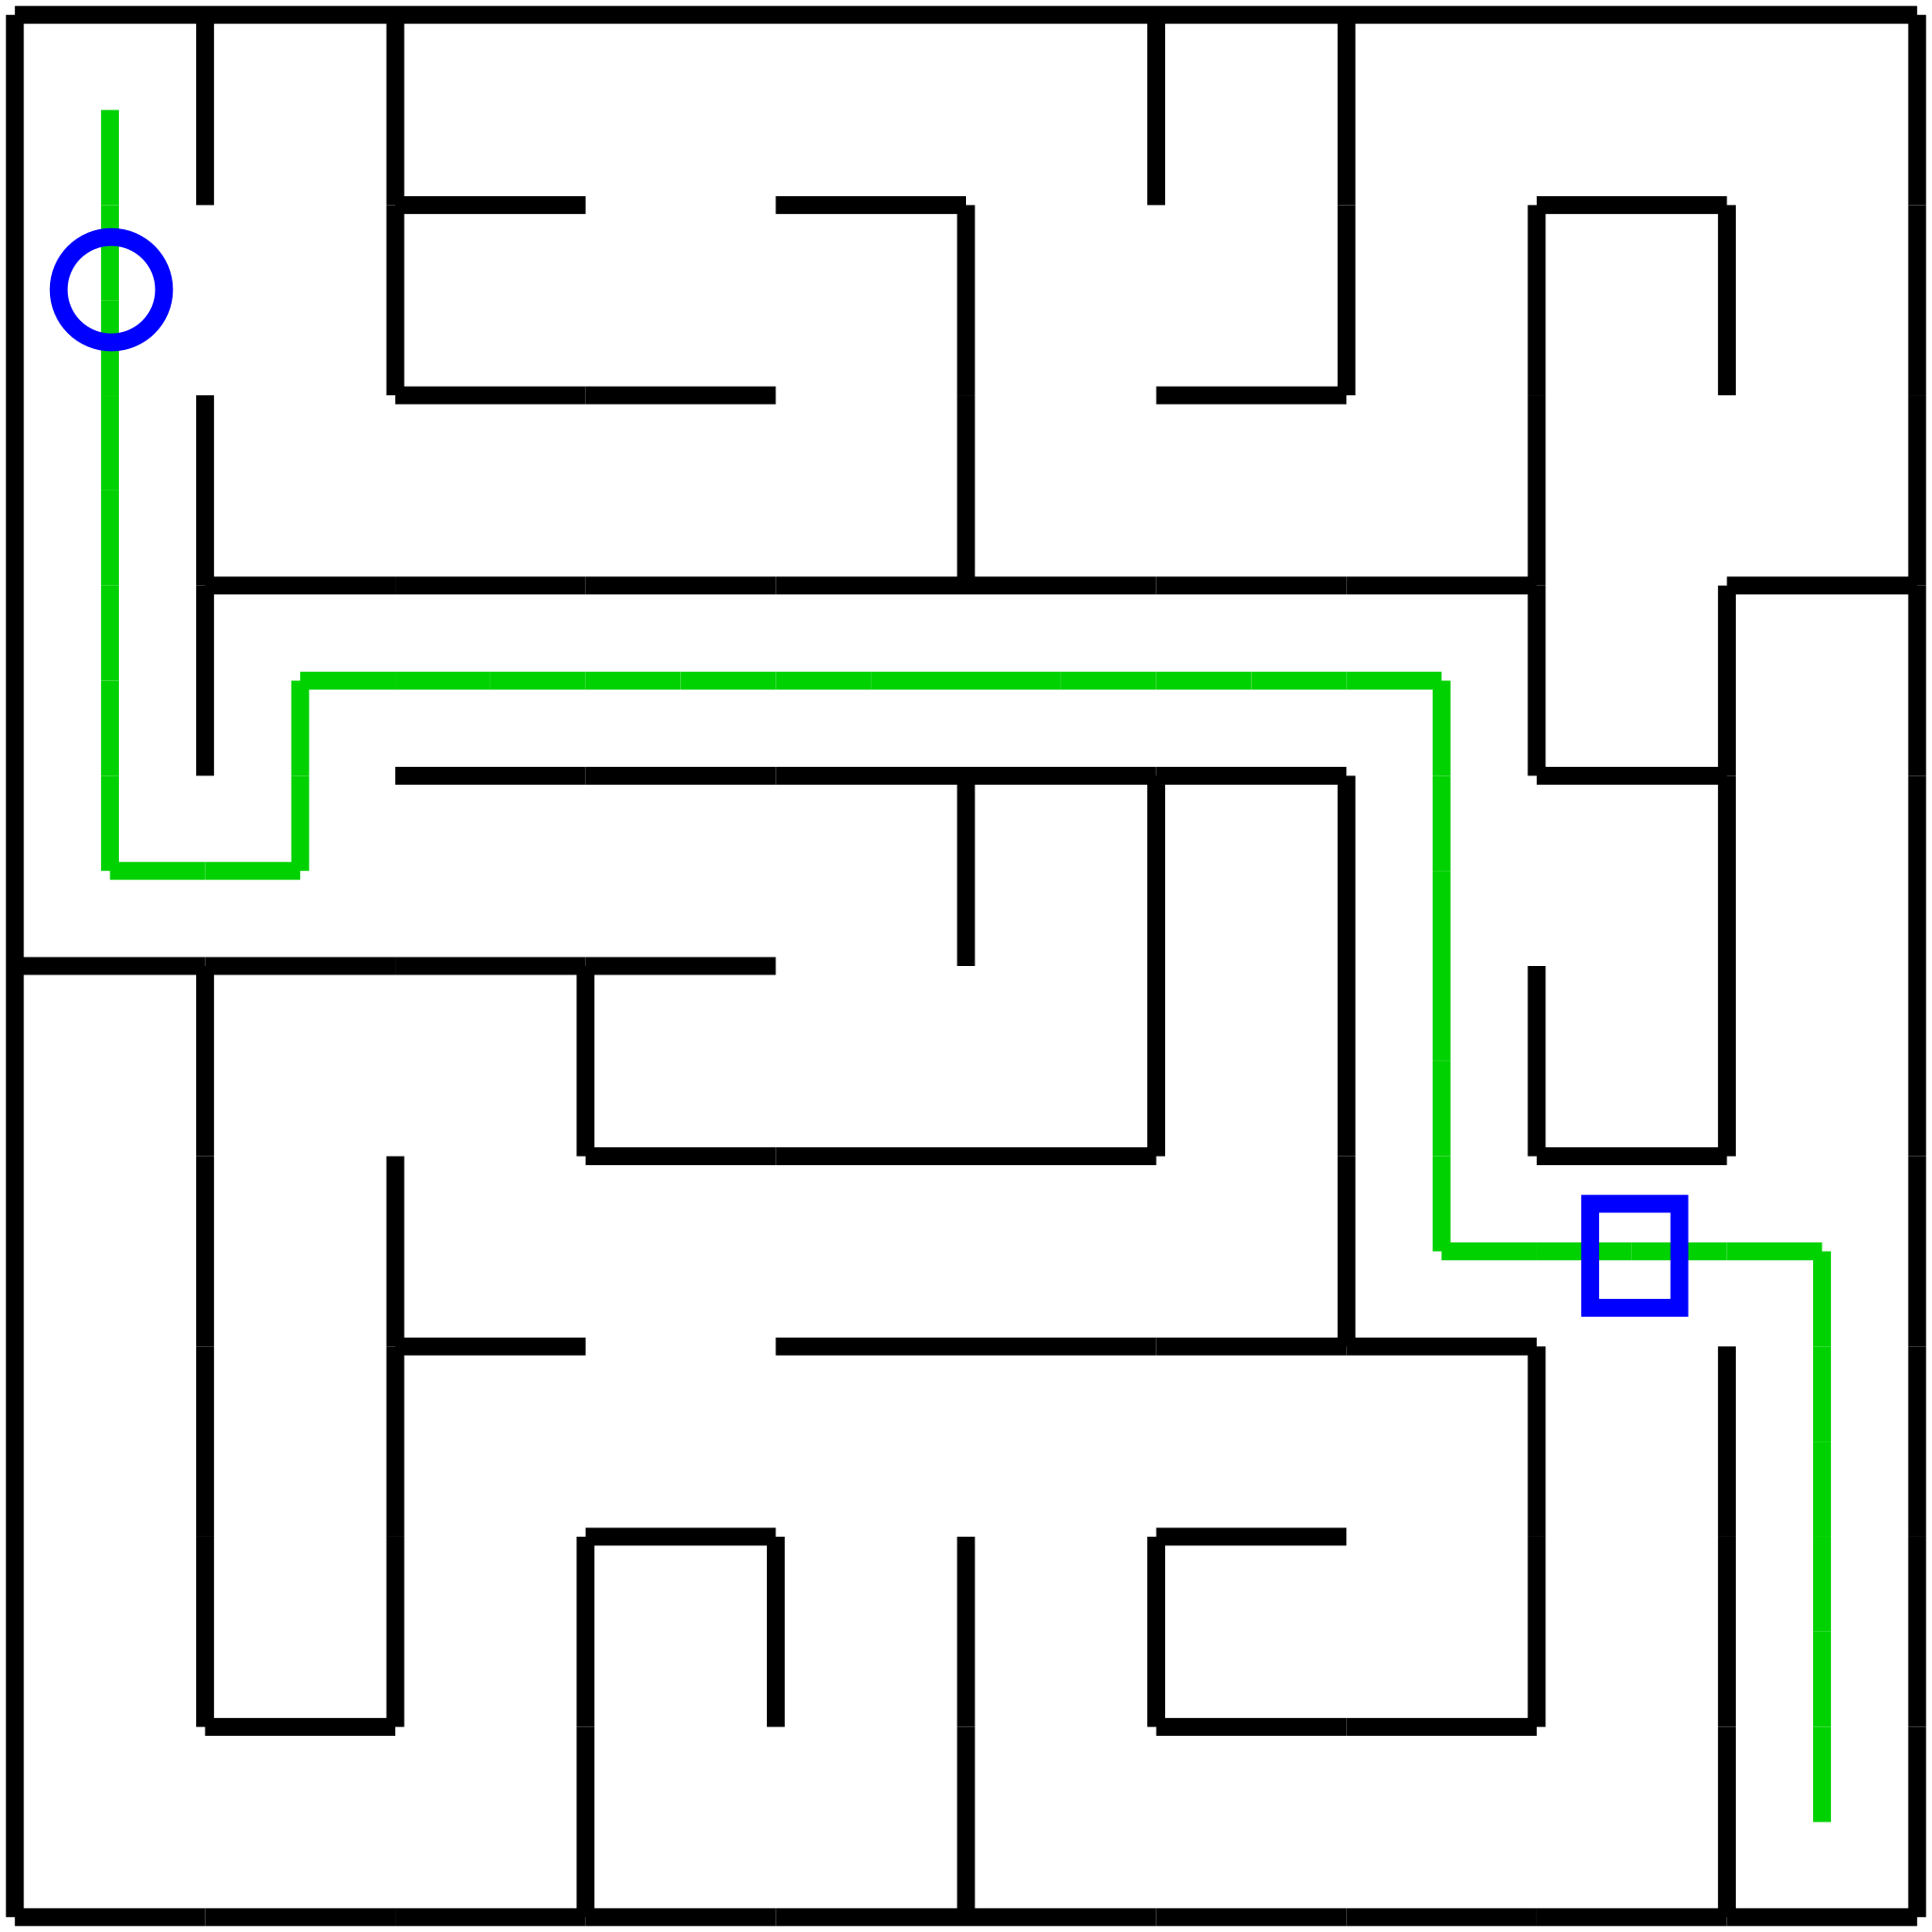
\includegraphics{SMPdesign/maze_in_way10a}}
\caption{Reason for Small Visit Percentages}
\label{fig:SMPdesign:Reason for Small Visit Percentages}
\end{figure}

\begin{figure}[tb]
\centering
\resizebox{2.2in}{!}{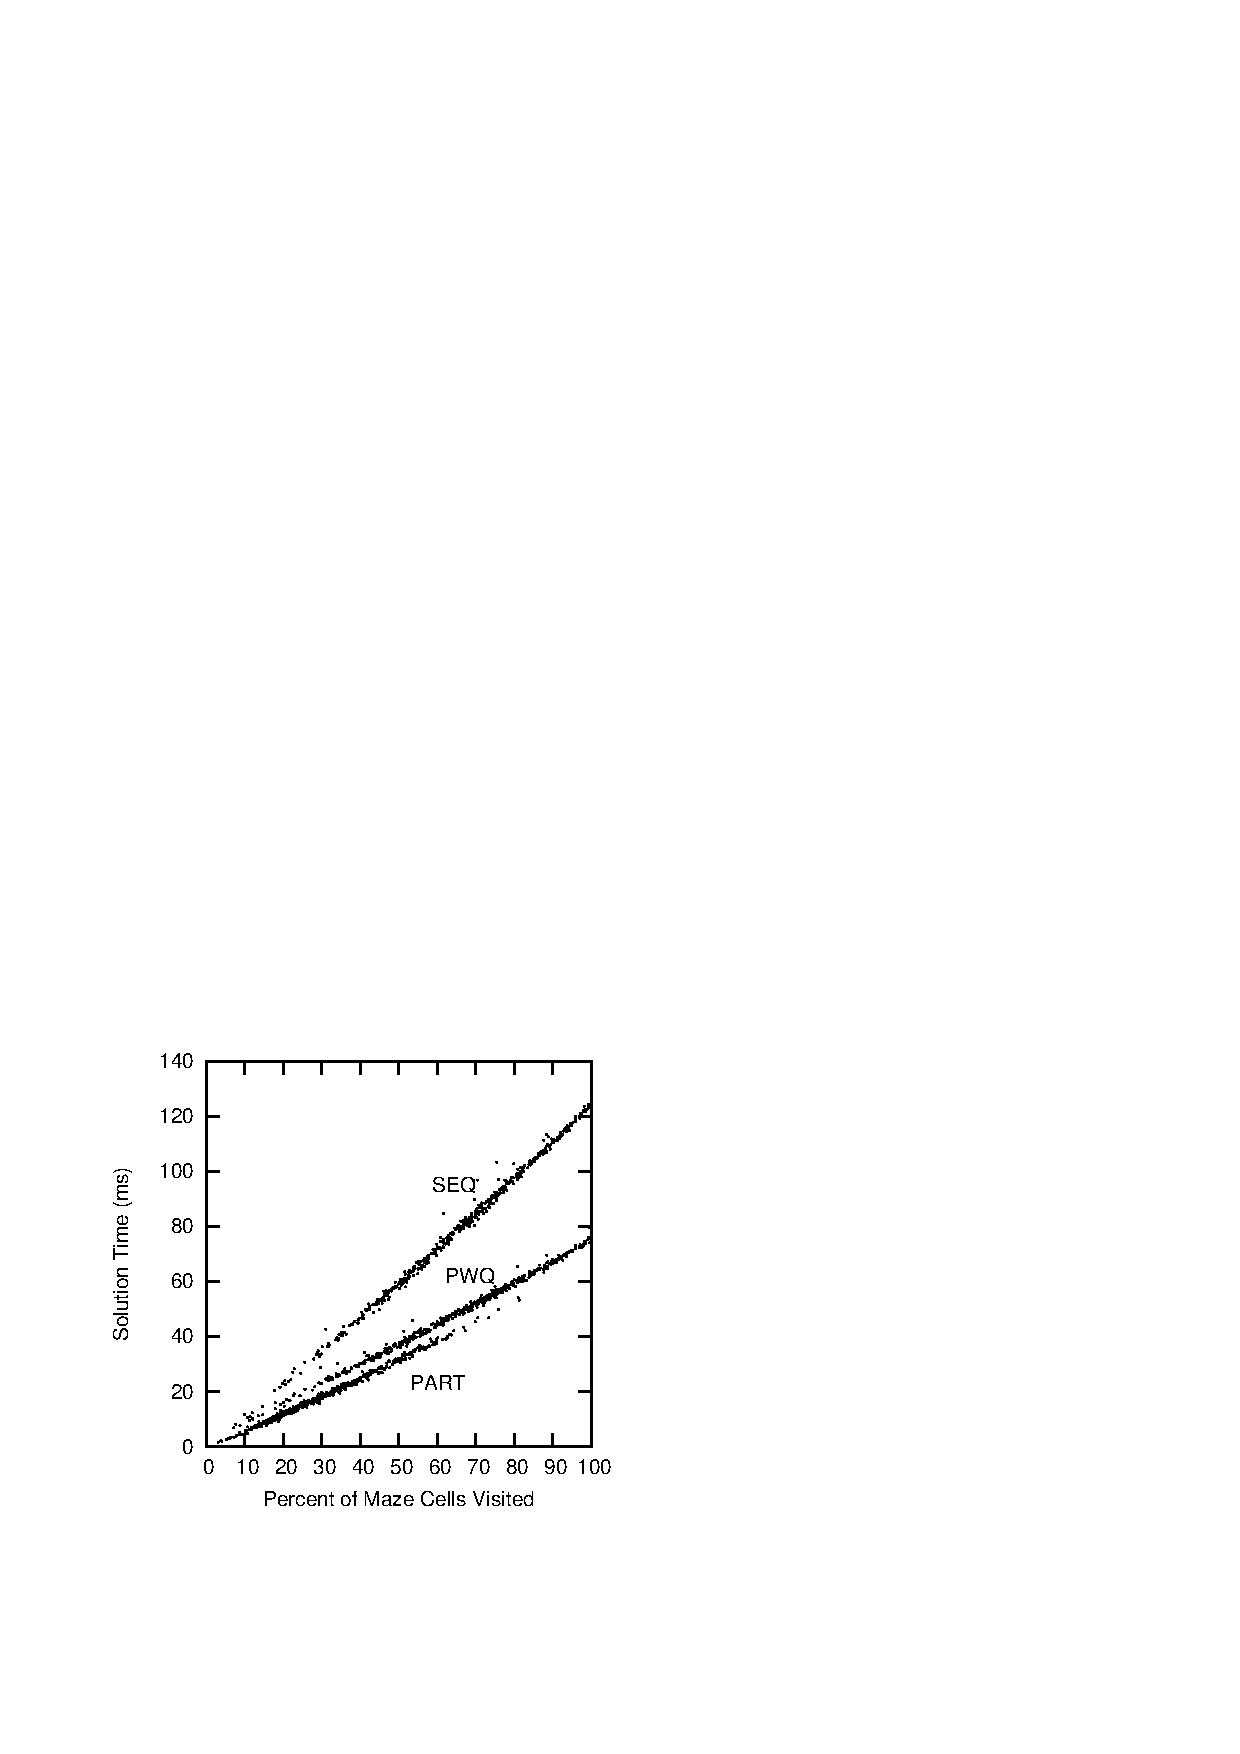
\includegraphics{SMPdesign/500-pctVms_seq_part-sct}}
\caption{Correlation Between Visit Percentage and Solution Time}
\label{fig:SMPdesign:Correlation Between Visit Percentage and Solution Time}
\end{figure}

더 나아가서 들여다본 결과 PART 는 가끔 미로의 셀들 중 2\,\% 미만만을 방문했는데,
SEQ 와 PWQ 는 9\,\% 미만을 방문한 적이 없었습니다.
이런 차이점에 대한 이유는
Figure~\ref{fig:SMPdesign:Reason for Small Visit Percentages} 에 보여져
있습니다.
만약 좌상당부터 시작해서 해결책을 찾는 쓰레드가 원에 도달하면 다른 쓰레드는
미로의 우상단에 도락할 수 없습니다.
비슷하게, 만약 다른 쓰레드가 네모에 도달하면, 첫번째 쓰레드는 미로의 좌하단에
도착할 수 없습니다.
따라서, PART 는 해법이 아닌 셀들로 이루어진 경로 중 더 작은 부분만을 방문하게
될 것입니다.
한마디로, 선형을 초월하는 속도 향상은 쓰레드들이 서로의 길을 만들어 주기
때문입니다.
이는 일하는 쓰레드들이 쓰레드들 각자의 길에서 다른 쓰레드들을 벗어나게 하기
위해 노력해왔던 수십년의 병렬 프로그래밍의 경험에 상당히 반대되는 이야기입니다.
\iffalse

Further investigation showed that
PART sometimes visited fewer than 2\,\% of the maze's cells,
while SEQ and PWQ never visited fewer than about 9\,\%.
The reason for this difference is shown by
Figure~\ref{fig:SMPdesign:Reason for Small Visit Percentages}.
If the thread traversing the solution from the upper left reaches
the circle, the other thread cannot reach
the upper-right portion of the maze.
Similarly, if the other thread reaches the square,
the first thread cannot reach the lower-left
portion of the maze.
Therefore, PART will likely visit a small fraction
of the non-solution-path cells.
In short, the superlinear speedups are due to threads getting in each
others' way.
This is a sharp contrast with decades of experience with
parallel programming, where workers have struggled
to keep threads \emph{out} of each others' way.
\fi

Figure~\ref{fig:SMPdesign:Correlation Between Visit Percentage and Solution Time}
는 세개의 모든 방법들에 대해 방문된 셀들의 수와 해결책 탐색에 걸리는 시간
사이의 강한 상관관계를 확실히 보여주고 있습니다.
PART 의 그림의 경사도는 SEQ 의 그것에 비해 작은데, 이것이 PART 의 쓰레드들이
SEQ 의 단일 쓰레드에 비해 미로의 주어진 부분을 더 빠르게 방문할 것임을 이야기
합니다.
PART 의 그림은 또한 작은 방문 퍼센티지에 몰려 있는데, 이는 PART 가 더 적은 일을
하게 되며, 따라서 관측된 굴욕적인 병렬성을 보이게 되는 것입니다.
\iffalse

Figure~\ref{fig:SMPdesign:Correlation Between Visit Percentage and Solution Time}
confirms a strong correlation between cells visited and solution time
for all three methods.
The slope of PART's scatterplot is smaller than that of SEQ,
indicating that PART's pair of threads visits a given fraction
of the maze faster than can SEQ's single thread.
PART's scatterplot is also weighted toward small visit
percentages, confirming that PART does less total work, hence
the observed humiliating parallelism.
\fi

\begin{figure}[tb]
\centering
\resizebox{1.4in}{!}{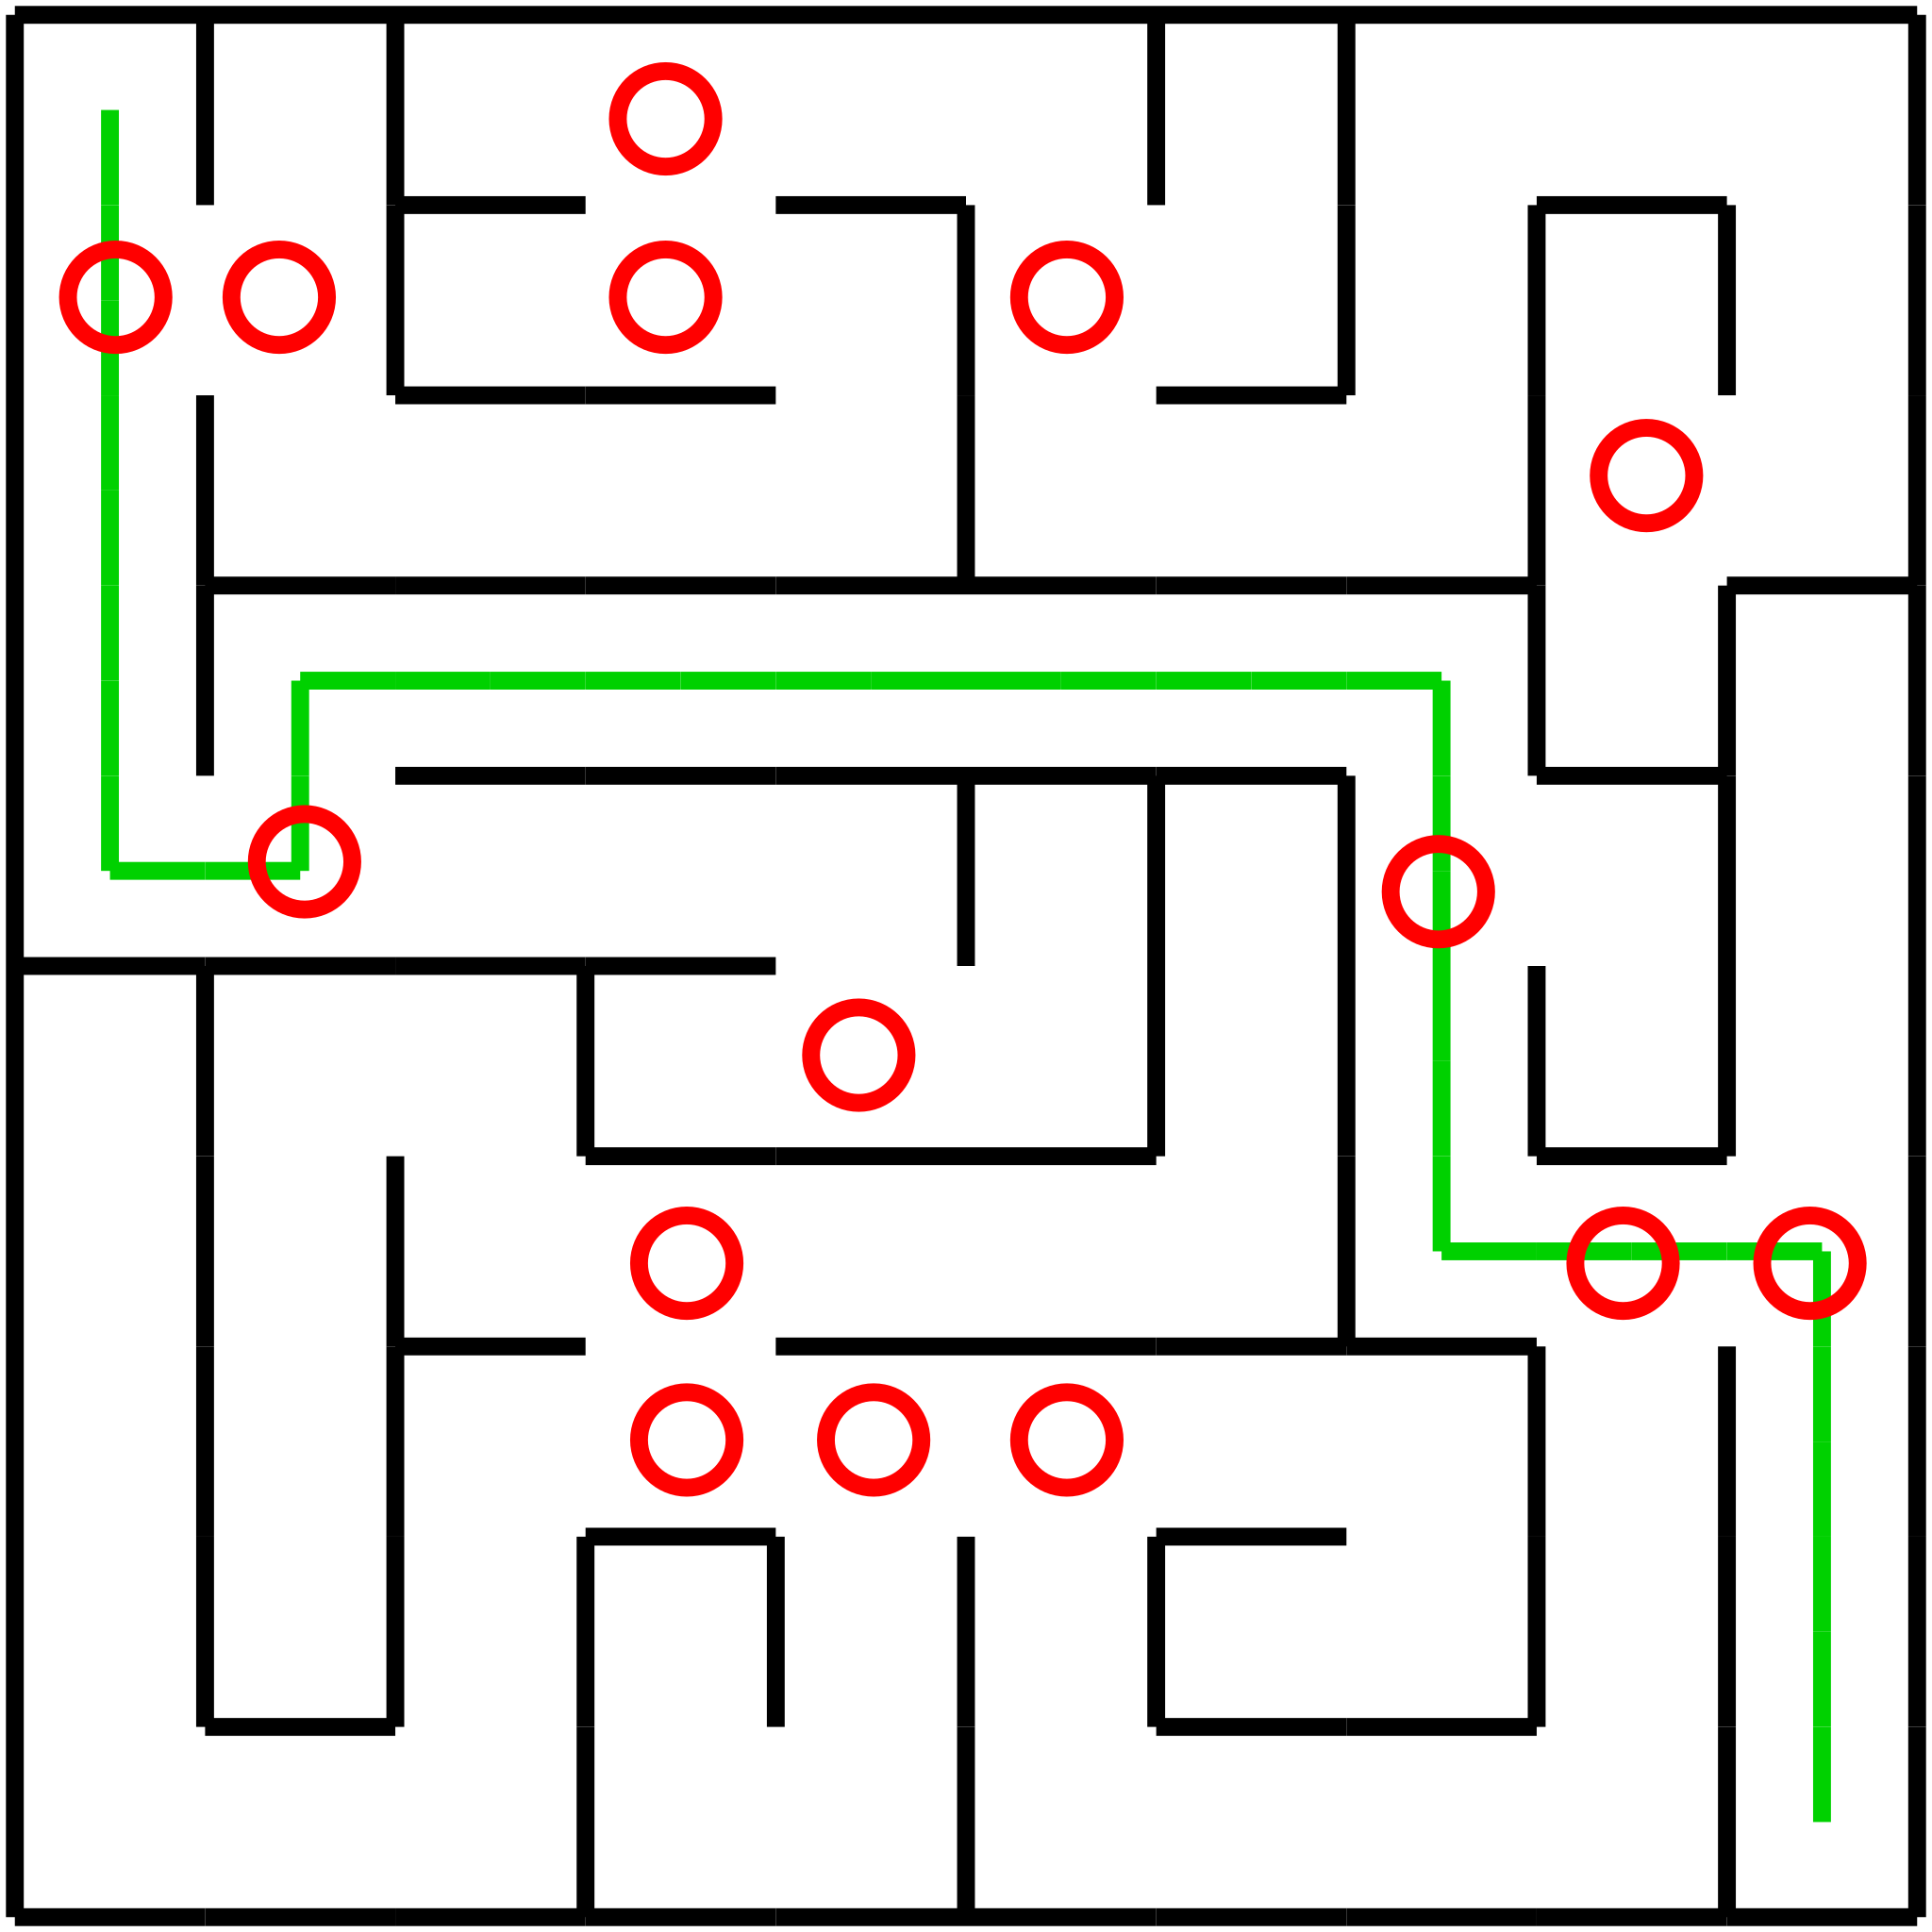
\includegraphics{SMPdesign/maze_PWQ_vs_PART}}
\caption{PWQ Potential Contention Points}
\label{fig:SMPdesign:PWQ Potential Contention Points}
\end{figure}

PWQ 에 의해 방문되는 셀들로 이루어진 부분들은 SEQ 의 그것과 유사합니다.
또한, PWQ 의 해결책 탐색에 걸리는 시간은 동일한 방문 부분들에도 불구하고 PART
의 그것에 비해 훨씬 큽니다.
이에 대한 이유가 Figure~\ref{fig:SMPdesign:PWQ Potential Contention Points} 에
그려져 있는데, 이 그림에는 두개 이상의 이웃을 가지고 있는 셀마다 붉은 원을
그려두었습니다.
그러한 각각의 셀은 PWQ 에서 경쟁 상황을 초래할 수 있는데, 한 쓰레드는 들어갈 수
있지만 두 쓰레드들이 나갈 수 있기 때문에, 이 챕터의 앞부분에서 설명했듯이
성능을 악화시킬 수 있기 때문입니다.
반면에 PART 는 그런 경쟁상황을 한번만 일으키는데, 해법이 찾아졌을 때입니다.
물론, SEQ 는 경쟁상황은 일으키지 않습니다.
\iffalse

The fraction of cells visited by PWQ is similar to that of SEQ.
In addition, PWQ's solution time is greater than that of PART,
even for equal visit fractions.
The reason for this is shown in
Figure~\ref{fig:SMPdesign:PWQ Potential Contention Points}, which has a red
circle on each cell with more than two neighbors.
Each such cell can result in contention in PWQ, because
one thread can enter but two threads can exit, which hurts
performance, as noted earlier in this chapter.
In contrast, PART can incur such contention but once, namely
when the solution is located.
Of course, SEQ never contends.
\fi

\begin{figure}[tb]
\centering
\resizebox{2.2in}{!}{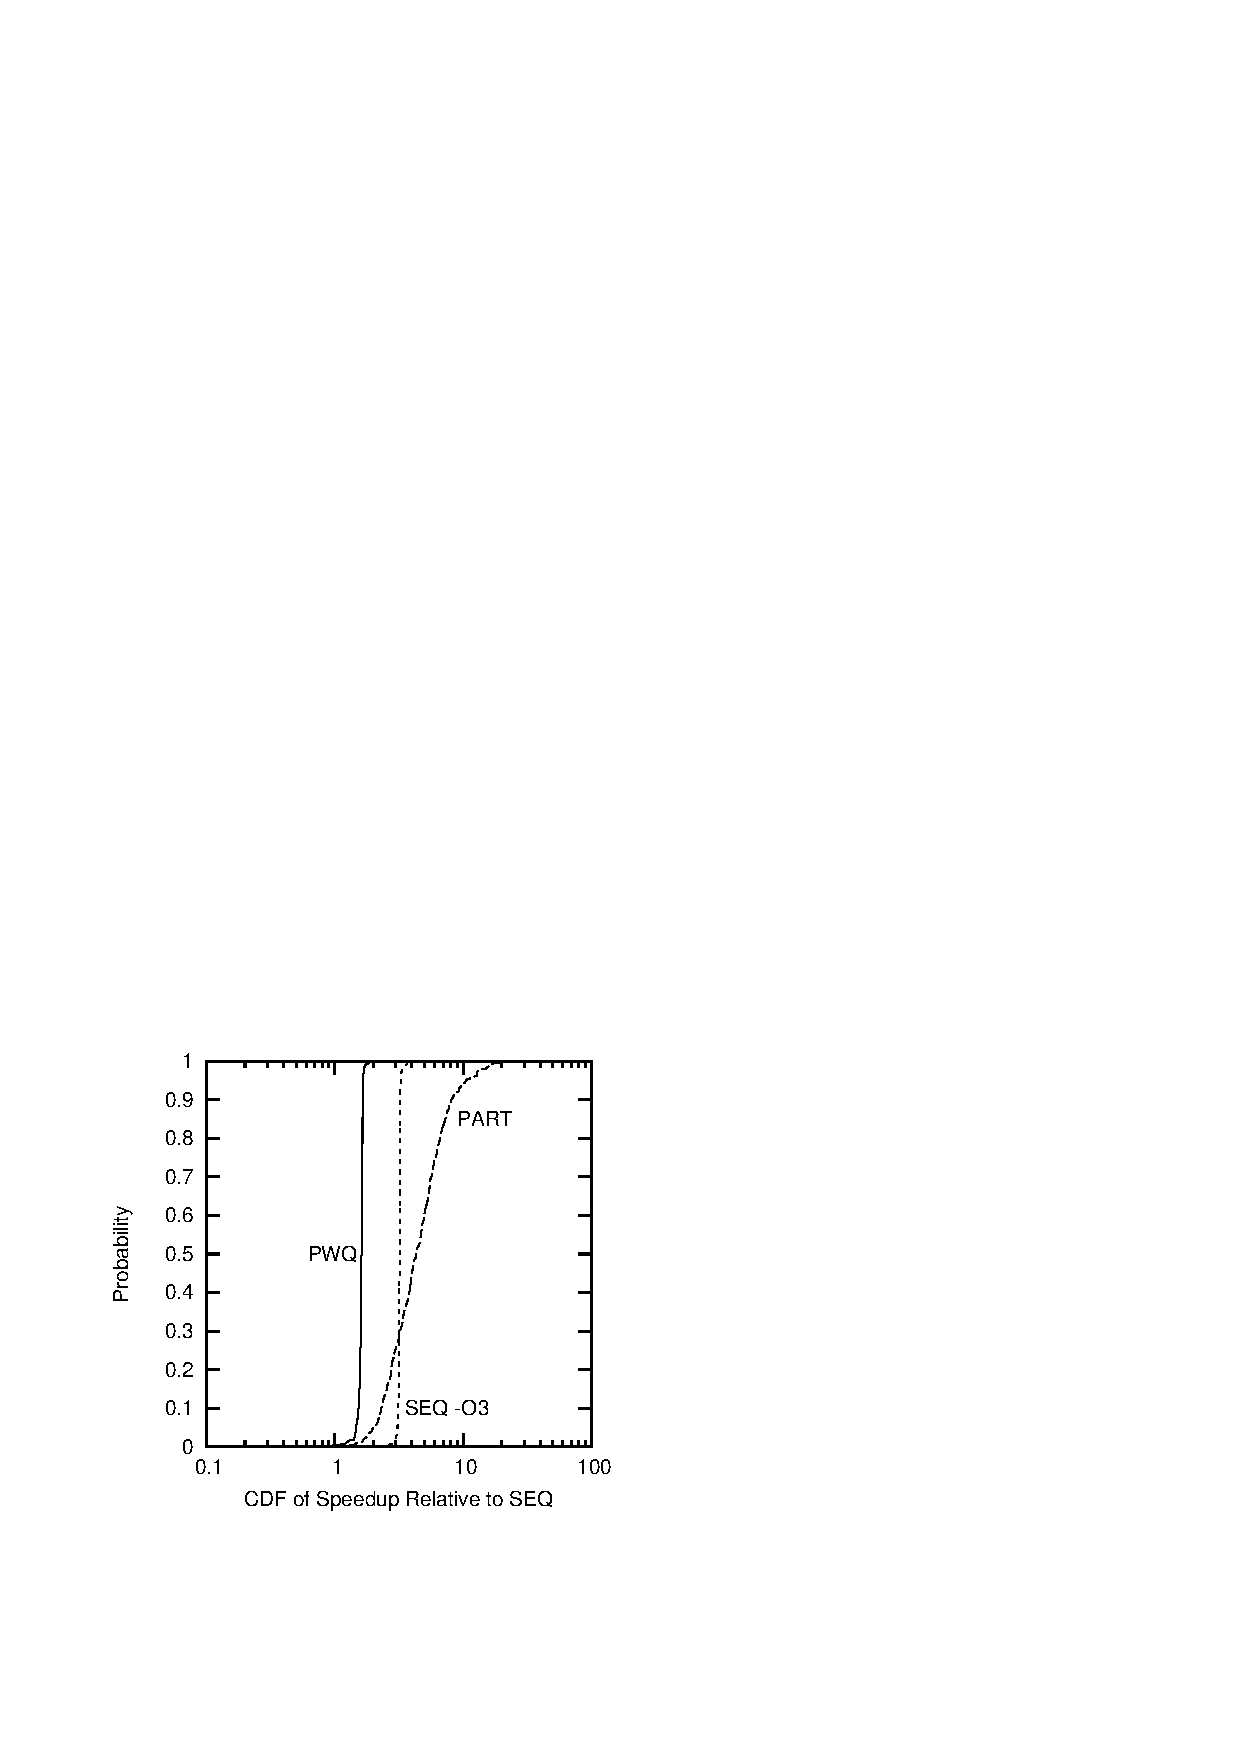
\includegraphics{SMPdesign/500-ms_seqVfg_part_seqO3-cdf}}
\caption{Effect of Compiler Optimization (-O3)}
\label{fig:SMPdesign:Effect of Compiler Optimization (-O3)}
\end{figure}

PART 의 성능 향상이 인상적이긴 하지만, 순차적인 최적화를 게을리 하지는 않아야
합니다.
Figure~\ref{fig:SMPdesign:Effect of Compiler Optimization (-O3)} 는 SEQ 가 -O3
옵션을 가지고 컴파일 되었을 때에는 최적화 되지 않은 PWQ 보다 두배 정도나
빠르고, 최적화 되지 않은 PART 의 성능에 근접합니다.
세개의 알고리즘을 모두 -O3 옵션을 주고 컴파일한 결과는 (더 빠르긴 하지만)
Figure~\ref{fig:SMPdesign:CDF of SEQ/PWQ and SEQ/PART Solution-Time Ratios} 에
보여진 그것들과 비슷한 양상을 보입니다만, PWQ 가 SEQ 에 비해 속도향상을 거의
보이지 않는다는 예외를 갖는데, 이는
Amdahl 의 법칙~\cite{GeneAmdahl1967AmdahlsLaw} 에 의함입니다.
하지만, 최적화 되지 않은 SEQ 에 비해 두배의 속도를 갖는게 목표라면, 컴파일러
최적화는 상당히 매력적인 방법이라 할 수 있겠습니다.
\iffalse

Although PART's speedup is impressive, we should not neglect sequential
optimizations.
Figure~\ref{fig:SMPdesign:Effect of Compiler Optimization (-O3)} shows that
SEQ, when compiled with -O3, is about twice as fast
as unoptimized PWQ, approaching the performance of unoptimized PART.
Compiling all three algorithms with -O3 gives results similar to
(albeit faster than) those shown in
Figure~\ref{fig:SMPdesign:CDF of SEQ/PWQ and SEQ/PART Solution-Time Ratios},
except that PWQ provides almost no speedup compared
to SEQ, in keeping with Amdahl's Law~\cite{GeneAmdahl1967AmdahlsLaw}.
However, if the goal is to double performance compared to unoptimized
SEQ, as opposed to achieving optimality, compiler
optimizations are quite attractive.
\fi

캐시 정렬과 패딩이 종종 거짓 공유 (false sharing) 을 줄여서 성능을 개선시키곤
합니다.
하지만, 이 미로 해법 알고리즘들에 있어서는, 미로 셀 배열에 정렬과 패딩을
적용하는 것은 1000x1000 미로에 대해 42\,\% 까지 성능을 \emph{떨어뜨립니다}.
캐시 로컬리티는 거짓 공유를 없애는 것보다 더 중요한데, 특히나 큰 미로에선 더욱
그러합니다.
작은 20x20 이나 50x50 미로에서라면, 정렬과 패딩이 PART 에 대해 성능을 40\,\% 까지
향상시킬 수 있습니다만 이런 작은 크기의 미로에 대해서는 PART 가 쓰레드를
생성하고 소멸시키는데 드는 오버헤드를 상쇄시키기에 충분한 시간을 갖지 못하기에
SEQ 가 더 좋은 성능을 보입니다.

정리하자면, 파티셔닝을 사용한 병렬 미로 해결책은 알고리즘적으로 선형을 초월한
속도향상의 하나의 재미있는 예입니다.
만약 ``알고리즘적으로 선형을 초월한 속도 향상'' 이 인지 부조화를 일으킨다면,
다음 섹션으로 넘어가 보시기 바랍니다.
\iffalse

Cache alignment and padding often improves performance by reducing
false sharing.
However, for these maze-solution algorithms, aligning and padding the
maze-cell array \emph{degrades} performance by up to 42\,\% for 1000x1000 mazes.
Cache locality is more important than avoiding
false sharing, especially for large mazes.
For smaller 20-by-20 or 50-by-50 mazes, aligning and padding can produce
up to a 40\,\% performance improvement for PART,
but for these small sizes, SEQ performs better anyway because there
is insufficient time for PART to make up for the overhead of
thread creation and destruction.

In short, the partitioned parallel maze solver is an interesting example
of an algorithmic superlinear speedup.
If ``algorithmic superlinear speedup'' causes cognitive dissonance,
please proceed to the next section.
\fi

\subsection{Alternative Sequential Maze Solver}
\label{sec:SMPdesign:Alternative Sequential Maze Solver}

\begin{figure}[tb]
\centering
\resizebox{2.2in}{!}{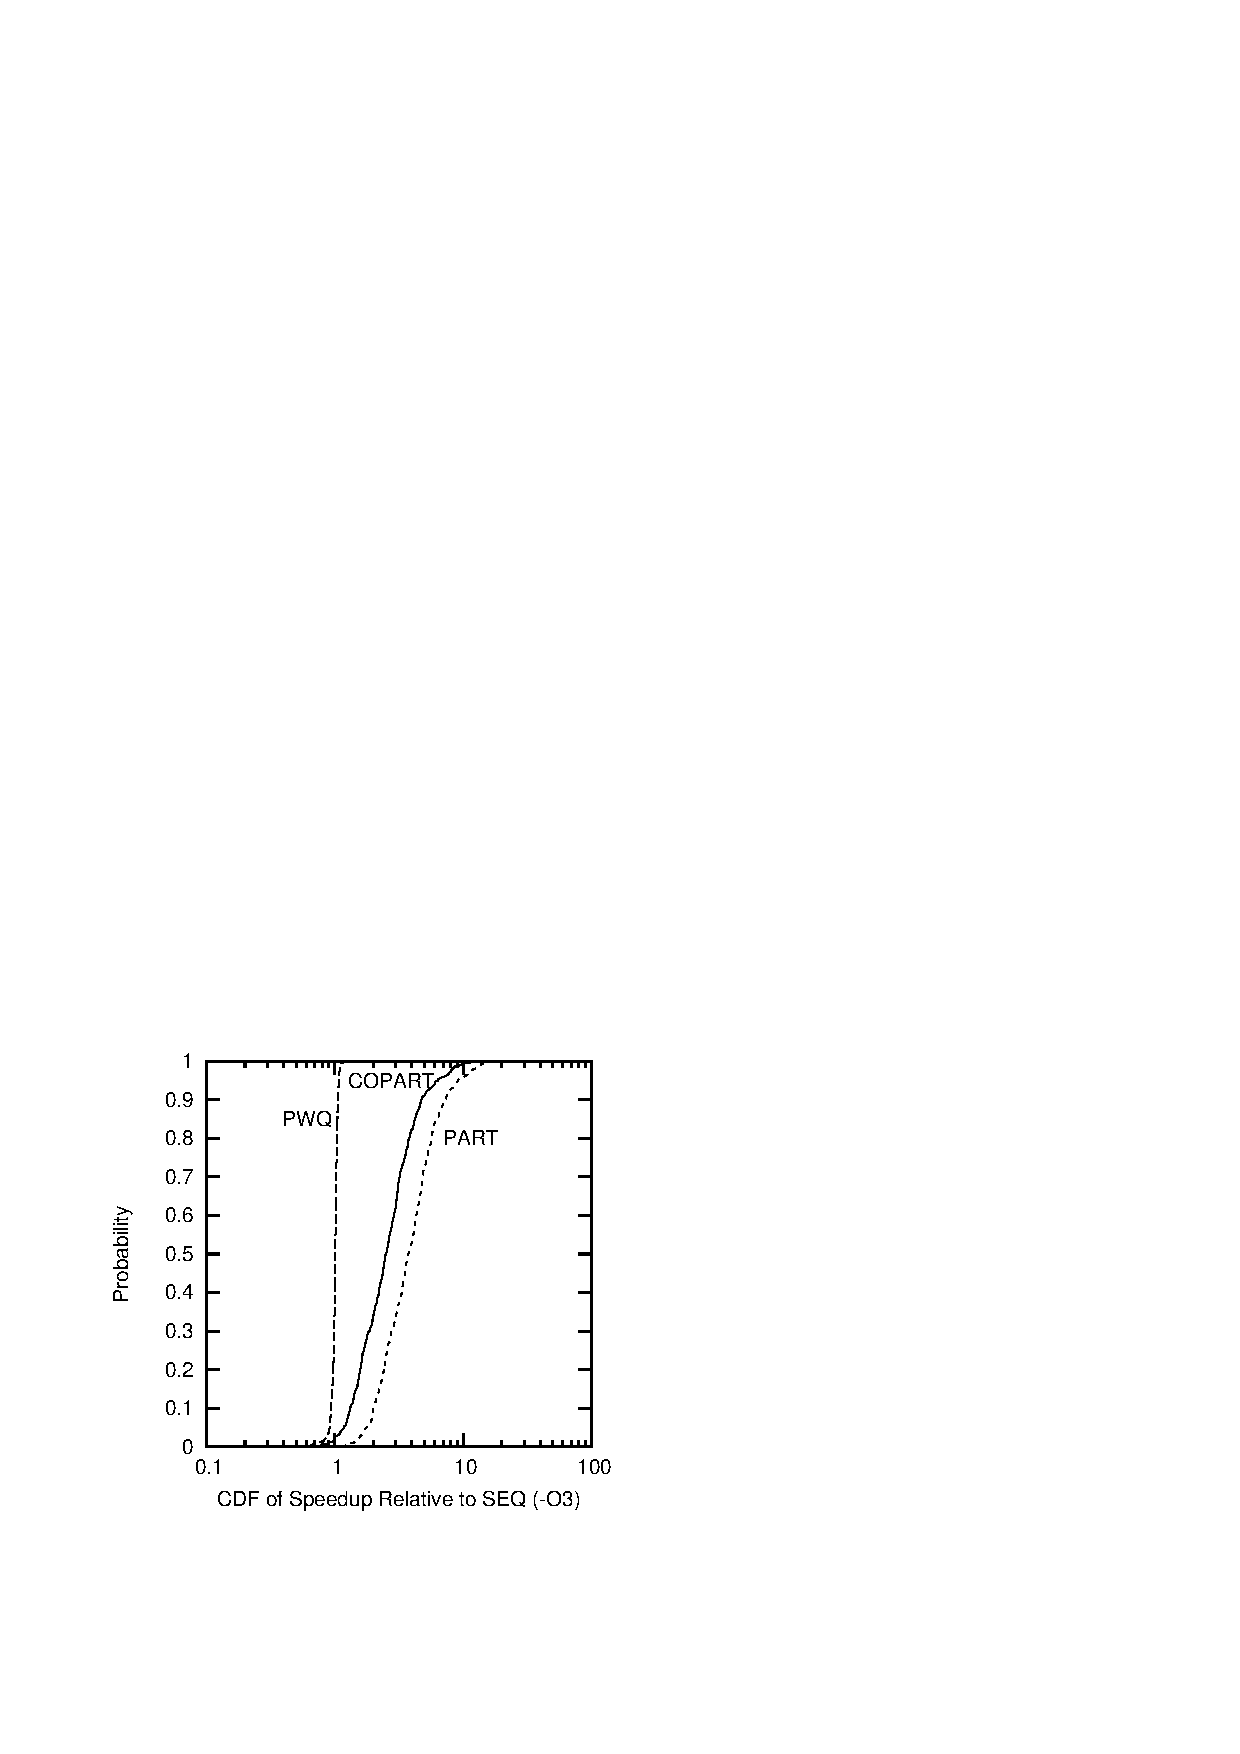
\includegraphics{SMPdesign/500-ms_seqO3V2seqO3_fgO3_partO3-cdf}}
\caption{Partitioned Coroutines}
\label{fig:SMPdesign:Partitioned Coroutines}
\end{figure}

알고리즘적으로 선형을 초월한 속도 향상의 존재는 코루틴 (co-routine) 을 통한
병렬성 모의실험을 제시하는데, 예를 들어, Listing~\ref{lst:SMPdesign:Partitioned
Parallel Solver Pseudocode} 의 do-while 루프의 각 패스에서 수동으로 컨텍스트
스위칭을 해보는 겁니다.
이 컨텍스트 스위칭은 직접적인데 이 컨텍스트는 변수들 \co{c} 와 \co{vi} 로만
구성되어 있기 때문입니다: 이 효과를 낼 수 있는 많은 방법들 중, 이 방법이
컨텍스트 스위칭 오버헤드와 방문 퍼센티지 사이의 좋은 트레이드오프입니다.
Figure~\ref{fig:SMPdesign:Partitioned Coroutines} 에서 볼 수 있듯이 이 코루틴
알고리즘 (COPART) 은 상당히 효과적으로, 한 쓰레드에서의 성능이 두 쓰레드를
사용한 PART 의 30\,\% 입니다(\co{maze_2seq.c}).
\iffalse

The presence of algorithmic superlinear speedups suggests simulating
parallelism via co-routines, for example, manually switching context
between threads on each pass through the main do-while loop in
Listing~\ref{lst:SMPdesign:Partitioned Parallel Solver Pseudocode}.
This context switching is straightforward because the context
consists only of the variables \co{c} and \co{vi}: Of the numerous
ways to achieve the effect, this is a good tradeoff between
context-switch overhead and visit percentage.
As can be seen in
Figure~\ref{fig:SMPdesign:Partitioned Coroutines},
this coroutine algorithm (COPART) is quite effective, with the performance
on one thread being within about 30\,\% of PART on two threads
(\path{maze_2seq.c}).
\fi

\subsection{Performance Comparison II}
\label{sec:SMPdesign:Performance Comparison II}

\begin{figure}[tb]
\centering
\resizebox{2.2in}{!}{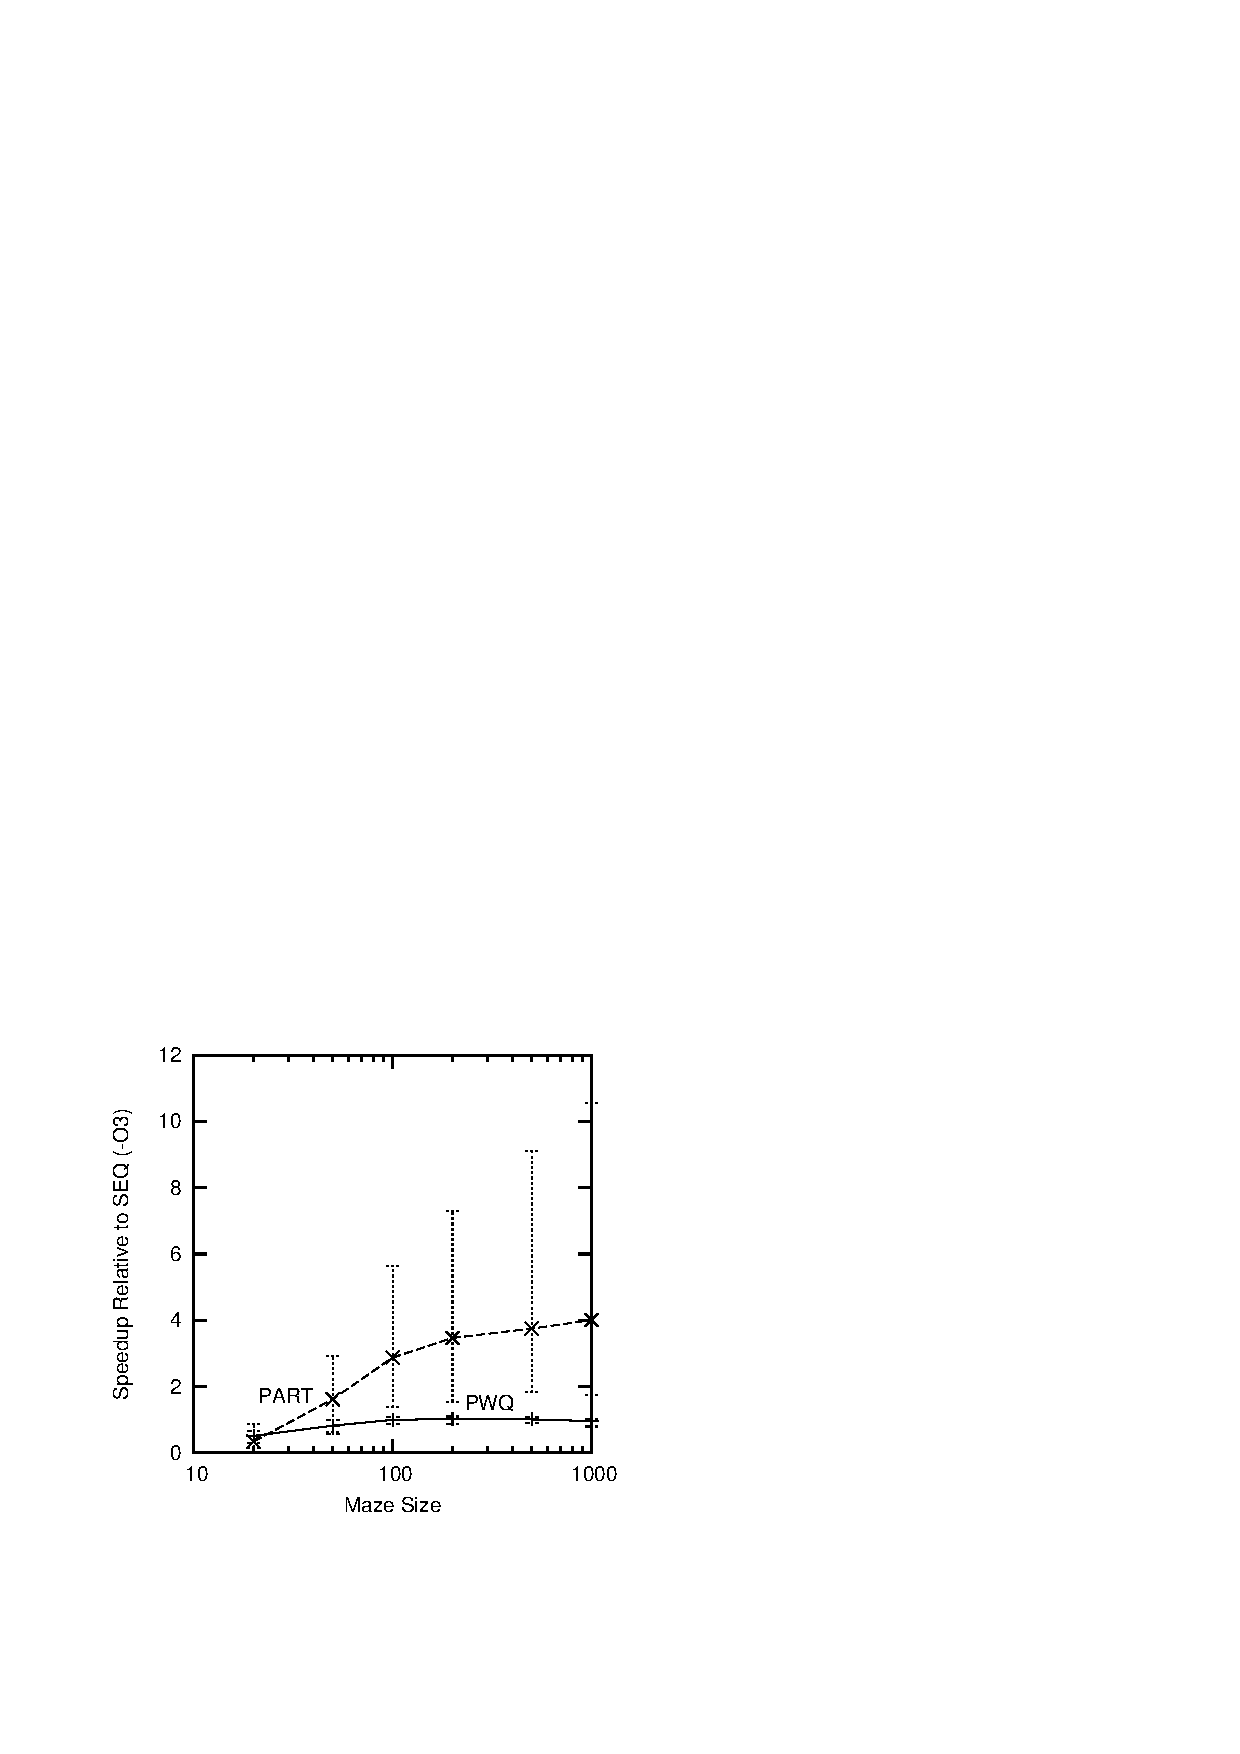
\includegraphics{SMPdesign/500-ms_seqO3VfgO3_partO3-median}}
\caption{Varying Maze Size vs. SEQ}
\label{fig:SMPdesign:Varying Maze Size vs. SEQ}
\end{figure}

\begin{figure}[tb]
\centering
\resizebox{2.2in}{!}{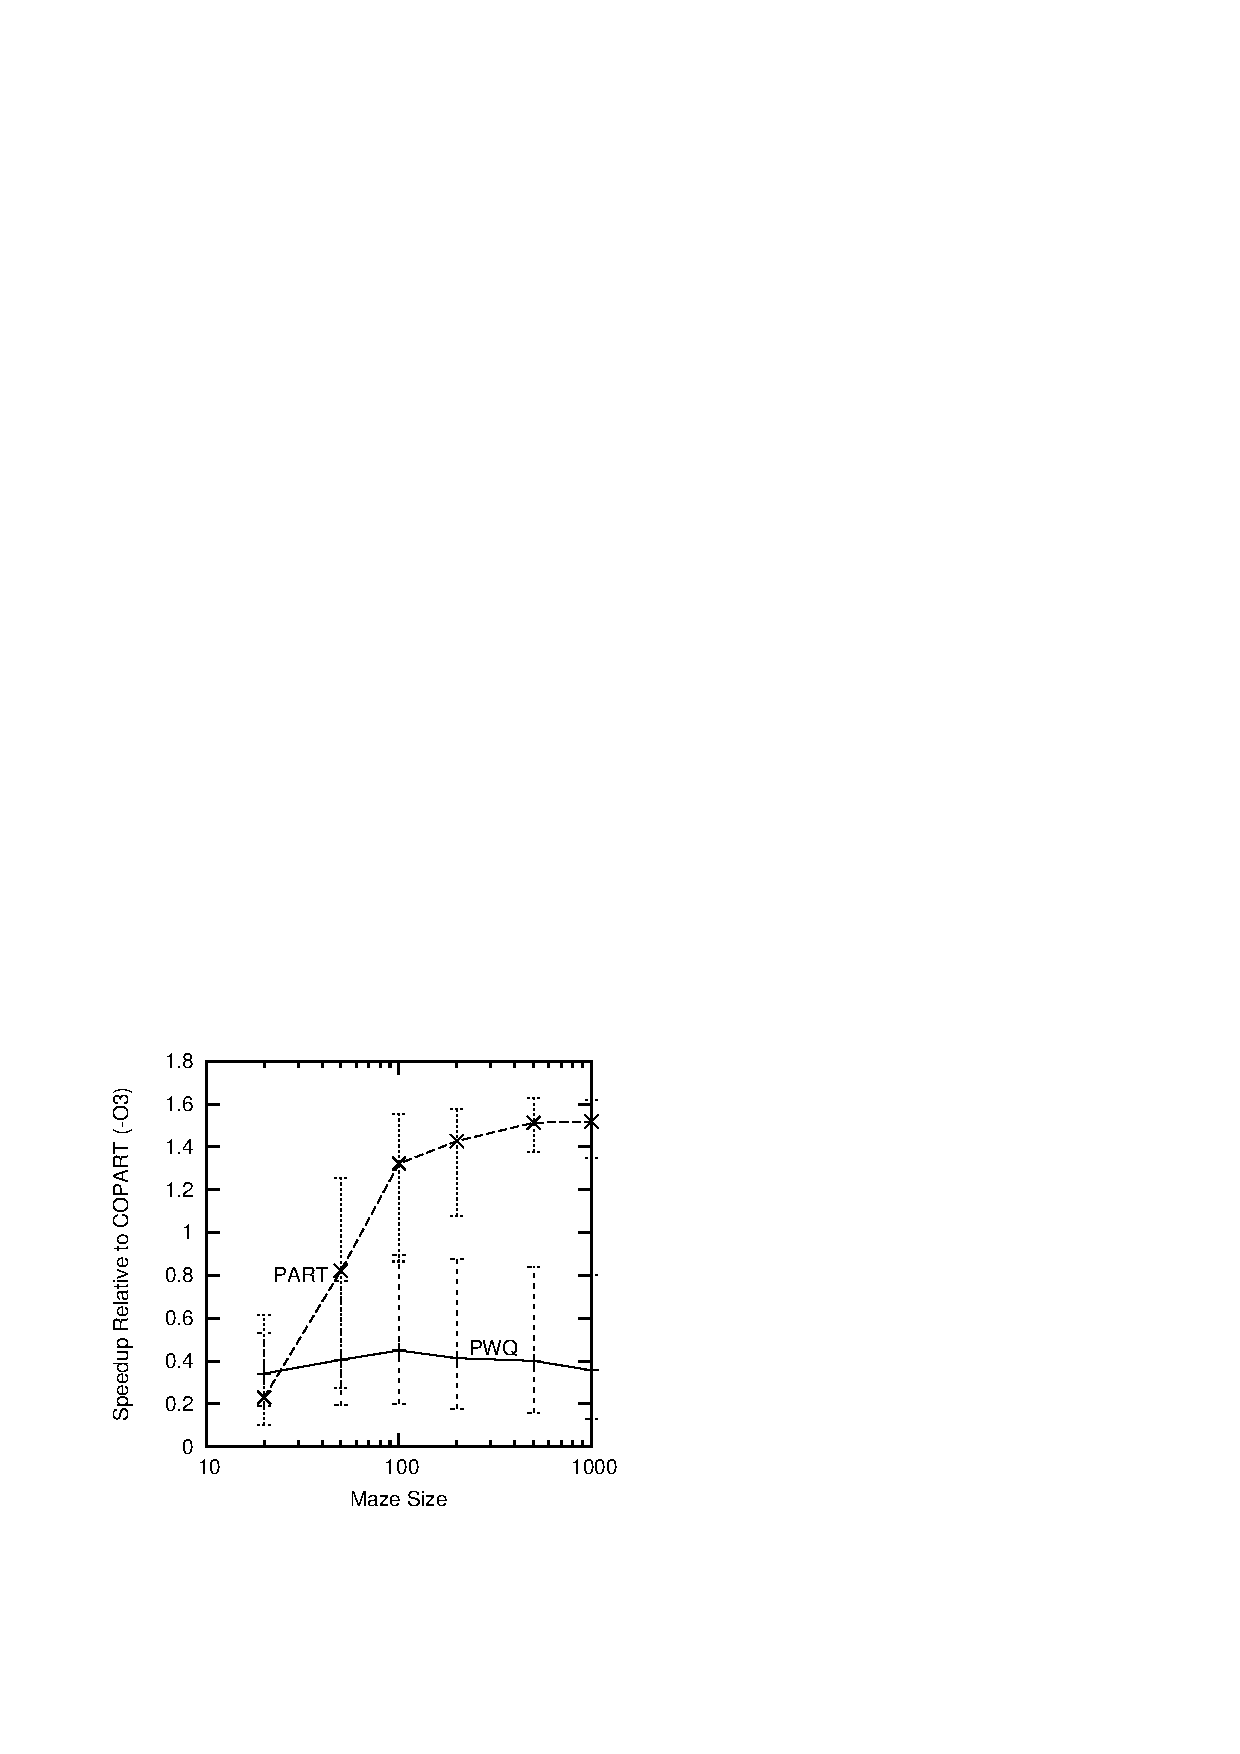
\includegraphics{SMPdesign/500-ms_2seqO3VfgO3_partO3-median}}
\caption{Varying Maze Size vs. COPART}
\label{fig:SMPdesign:Varying Maze Size vs. COPART}
\end{figure}

Figures~\ref{fig:SMPdesign:Varying Maze Size vs. SEQ}
와~\ref{fig:SMPdesign:Varying Maze Size vs. COPART} 는 미로의 크기의 변화에
따른 효과를 두개의 쓰레드로 동작하는 PWQ 와 PART 를 SEQ 또는 COPART 와 각각
비교해 90\,\% 의 정확성 에러 막대와 함께 보여주고 있습니다.
PART 는 100행 100열 이상 크기의 미로들에서 SEQ 에 비해 선형성을 초월한 확장성을
보이고 COPART 에 비해서는 적당한 확장성을 보입니다.
에너지 소모가 높은 주파수에서는 대략 주파수의 제곱 정도로 증가한다는
가정~\cite{TrevorMudge2000Power} 에 기반해서 보면 두 쓰레드를 사용해서 1.4 배의
확장성을 갖는 것은 단일 쓰레드가 같은 해법 탐색 시간을 필요로 할 때 소모하는
에너지와 동일하므로 PART 는 COPART 에 비교했을때 대략 200행 200열 크기 미로에서
이론적인 에너지 효율성 손익분기를 넘어섭니다.
반면, PWQ 는 SEQ 에 대해서도 COPART 에 대해서도 빈약한 확장성을 보이는데, 이는
최적화가 적용되었을 때 이야기입니다: Figure~\ref{fig:SMPdesign:Varying Maze
Size vs. SEQ}
와~\ref{fig:SMPdesign:Varying Maze Size vs. COPART} 는 -O3 옵션을 사용해
만들어졌습니다.
\iffalse

Figures~\ref{fig:SMPdesign:Varying Maze Size vs. SEQ}
and~\ref{fig:SMPdesign:Varying Maze Size vs. COPART}
show the effects of varying maze size, comparing both PWQ and PART
running on two threads
against either SEQ or COPART, respectively, with 90\=/percent\-/confidence
error bars.
PART shows superlinear scalability against SEQ and modest scalability
against COPART for 100-by-100 and larger mazes.
PART exceeds theoretical energy-efficiency breakeven against COPART at roughly
the 200-by-200 maze size, given that power consumption rises as roughly
the square of the frequency for high frequencies~\cite{TrevorMudge2000Power},
so that 1.4x scaling on two threads consumes the same energy
as a single thread at equal solution speeds.
In contrast, PWQ shows poor scalability against both SEQ and COPART
unless unoptimized: Figures~\ref{fig:SMPdesign:Varying Maze Size vs. SEQ} 
and~\ref{fig:SMPdesign:Varying Maze Size vs. COPART}
were generated using -O3.
\fi

\begin{figure}[tb]
\centering
\resizebox{2.2in}{!}{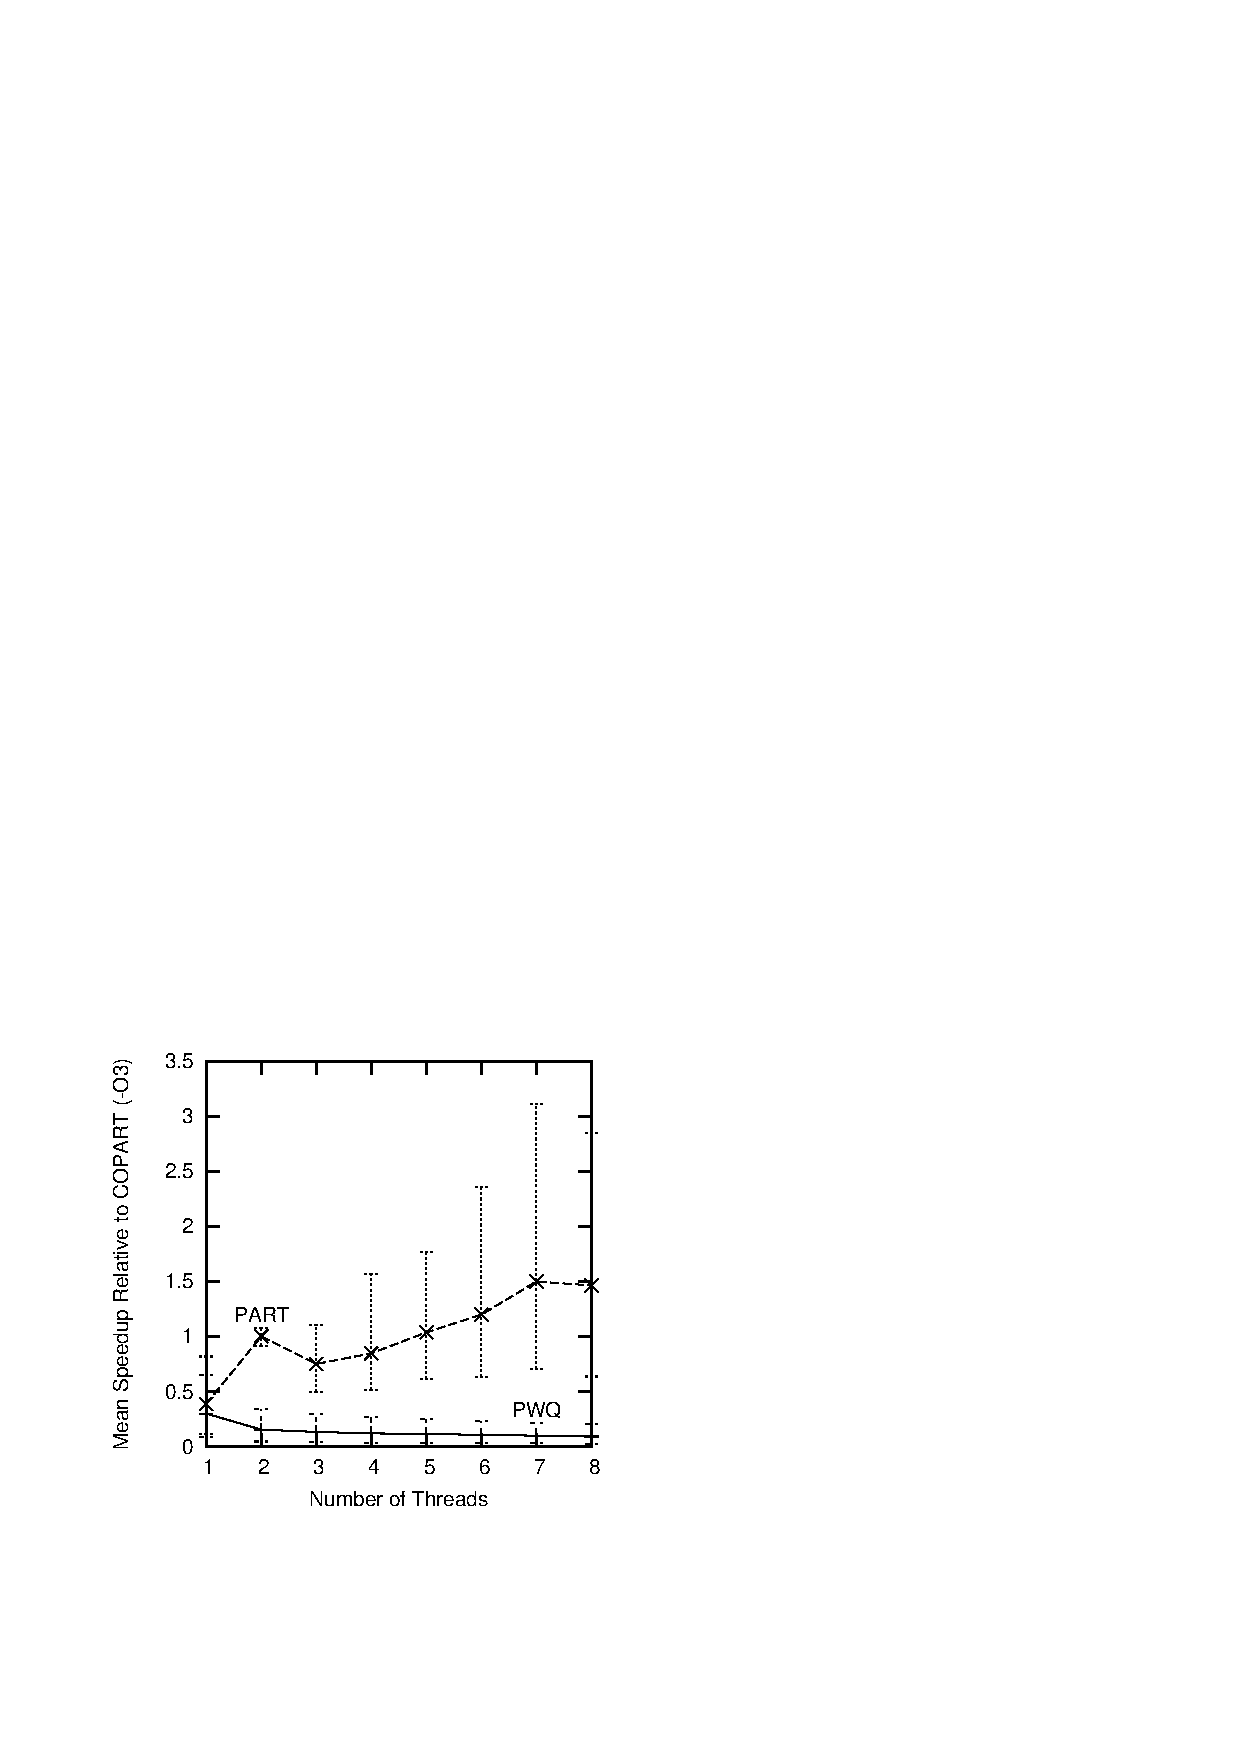
\includegraphics{SMPdesign/1000-ms_2seqO3VfgO3_partO3-mean}}
\caption{Mean Speedup vs. Number of Threads, 1000x1000 Maze}
\label{fig:SMPdesign:Mean Speedup vs. Number of Threads, 1000x1000 Maze}
\end{figure}

Figure~\ref{fig:SMPdesign:Mean Speedup vs. Number of Threads, 1000x1000 Maze}
는 PWQ 와 PART 의 성능을 COPART 에 비교해서 보여주고 있습니다.
두개가 넘는 쓰레드들을 사용해 동작하는 PART 의 경우, 추가된 쓰레드들은 미로의
시작점과 끝점 사이를 대각선으로 동일한 거리로 나뉘어진 위치에서부터 경로 탐색을
시작합니다.
두개가 넘는 쓰레드들을 사용해 동작하는 PART 의 이른 종료를 알아채기 위해서는
간략화된 링크 상태 라우팅~\cite{BERT-87} 이 사용되었습니다 (해법은 한 쓰레드가
시작점과 끝점과 연결되면 찾아진 것으로 표시됩니다).
PWQ 는 상당히 나쁜 성능 결과를 보입니다만, PART 는 두개 쓰레드에서, 그리고
다섯개 쓰레드에서 한번 더 손익분기에 도달하는데 다섯개 쓰레드를 넘어서고부터는
적당한 속도향상을 이루어냅니다.
이론적인 에너지 효율성 손익분기는 7개와 8개 쓰레드들에 대해서는 90\,\% 신뢰구간
안에 있습니다.
두개 쓰레드에서 성능이 뾰족하게 솟아오르는 이유는 (1) 두개 쓰레드의 경우의 덜
복잡한 해법 탐색 종료 파악 과정과 (2) 세번째와 그 뒤의 쓰레드들이 유용한 진전을
만들 확률이 좀 더 낮은 편이라는 사실입니다: 오직 처음의 두 쓰레드만이 해법의
경로에 직결됨이 보장됩니다.
Figure~\ref{fig:SMPdesign:Varying Maze Size vs. COPART} 에 비해 비교적
실망스러운 이 성능 결과는 2.66GHz 로 동작하는 더 크고 오래된
Xeon\textsuperscript\textregistered 에 사용되는 덜 밀접하게 융합된 하드웨어의
탓입니다.
\iffalse

Figure~\ref{fig:SMPdesign:Mean Speedup vs. Number of Threads, 1000x1000 Maze}
shows the performance of PWQ and PART relative to COPART.
For PART runs with more than two threads, the additional threads were
started evenly spaced along the diagonal connecting the starting and
ending cells.
Simplified link-state routing~\cite{BERT-87} was used to
detect early termination on PART runs with more than two threads
(the solution is flagged when
a thread is connected to both beginning and end).
PWQ performs quite poorly, but
PART hits breakeven at two threads and again at five threads, achieving
modest speedups beyond five threads.
Theoretical energy efficiency breakeven is within the 90\=/percent\-/confidence
interval for seven and eight threads.
The reasons for the peak at two threads are (1) the lower complexity
of termination detection in the two-thread case and (2) the fact that
there is a lower probability of the third and subsequent threads making
useful forward progress: Only the first two threads are guaranteed to start on
the solution line.
This disappointing performance compared to results in
Figure~\ref{fig:SMPdesign:Varying Maze Size vs. COPART}
is due to the less-tightly integrated hardware available in the
larger and older Xeon\mytextregistered\
system running at 2.66\,GHz.
\fi

\subsection{Future Directions and Conclusions}
\label{sec:SMPdesign:Future Directions and Conclusions}

너무 많은 해야할 일들이 남아있습니다.
첫째로, 이 섹션은 사람이 미로 해법 탐색 사용하는 방법 가운데 하나의 방법만을
적용해 보았습니다.
이외의 방법으로는 미로의 일부를 제거하기 위해 벽을 따라가는 방법과 이전에
탐색한 경로의 위치에 기반해서 내부 시작 지점을 고르는 방법 등이 있습니다.
둘째로, 시작지점과 끝지점의 다른 선택은 다른 알고리즘에 좀 더 효과적일 수
있습니다.
셋째로, PART 알고리즘의 첫번째 적용했던 방법인 두개 쓰레드 사용이 직선적이긴
하지만, 다른 여분의 쓰레드들을 사용하기 위한 방법들이 여럿 있습니다.
최적의 쓰레드 사용은 시작지점과 끝지점에도 의존적일 것입니다.
넷째로, 해결이 불가능한 미로들과 순환적인 미로들에 대한 연구는 재미있는 결과를
내놓을 수 있을 것입니다.
다섯째로, 가벼운 C++11 어토믹 오퍼레이션들은 성능을 개선시킬 수도 있습니다.
여섯째로, 3차원 미로 (또는 그보다도 높은 차원의 미로들) 의 속도 향상을 비교해
보는 것도 재미있을 것입니다.
마지막으로, 미로의 경우, 굴욕적 병렬성은 코루틴들을 사용한 보다 효과적인 순차적
구현을 의미했습니다.
굴욕적 병렬성 알고리즘은 항상 더 효과적인 순차적 구현을 이끌게 될까요, 아니면
코루틴 컨텍스트 스위치 오버헤드가 속도향상을 압도해버리는 고유의 굴욕적 병렬성
알고리즘이 존재할까요?
\iffalse

Much future work remains.
First, this section applied only one technique used by human maze solvers.
Others include following walls to exclude portions of the maze
and choosing internal starting points based on the
locations of previously traversed paths.
Second, different choices of
starting and ending points might favor different algorithms.
Third, although placement of the PART algorithm's
first two threads is straightforward, there are any number of
placement schemes for the remaining threads.
Optimal placement might well depend on the starting and ending points.
Fourth, study of unsolvable mazes and cyclic mazes
is likely to produce interesting results.
Fifth, the lightweight C++11 atomic operations might improve performance.
Sixth, it would be interesting to compare the speedups for
three-dimensional mazes (or of even higher-order mazes).
Finally, for mazes, humiliating parallelism indicated a
more-efficient sequential implementation using coroutines.
Do humiliatingly parallel algorithms always lead to more-efficient
sequential implementations, or are there inherently humiliatingly parallel
algorithms for which coroutine context-switch overhead overwhelms the
speedups?
\fi

이 섹션은 미로 해법 탐색 알고리즘들의 병렬화를 선보이고 분석해 보았습니다.
일반적인 일거리 대기열 기반의 알고리즘은 컴파일러 최적화가 꺼져있을 때에만 잘
동작했는데, 이는 기존에 고수준의/오버헤드가 많은 언어를 사용해 얻어졌던 결과들
중 일부는 진보된 최적화에 의해서 무효화 될수도 있음을 의미합니다.

이 섹션은 병렬화를 적용하는 것을 순차적 알고리즘의 파생물로 생각하기보다는
최적화를 위한 첫번째 선택지로 생각하는 것이 개선된 순차적 알고리즘을 위한 길의
기반을 닦음의 확연한 예 하나를 선보였습니다.
고수준 설계 레벨에서의 병럴성의 응용은 결실 있는 연구가 될 가능성이 큽니다.
이 섹션은 미로 탈출 경로를 탐색하는 문제를 느슨하게 확장성 있는 경우부터
굴욕적으로 병렬적인 경우까지 그리고 그 반대로도 풀어보았습니다.
이 경험이 병렬성에 기반한 작업을 무식하게 별로 최적이지 않은 경우가 많은, 이미
존재하는 프로그램에 개조의 형태로 적용되는 기존 성능 결과에 기반한 작은
최적화와 같은 것보다는 설계시점에서의 전체 어플리케이션을 위한 최적화 기법의
첫번째 선택지로 여겨지도록 하는데 동기를 부여하길 바랍니다.
\iffalse

This section demonstrated and analyzed parallelization of maze-solution
algorithms.
A conventional work-queue-based algorithm did well only when compiler
optimizations were disabled, suggesting that some prior results obtained
using high-level/overhead languages will be invalidated
by advances in optimization.

This section gave a clear example where approaching parallelism
as a first-class optimization technique rather than as a derivative of a
sequential algorithm paves the way for an improved sequential algorithm.
High-level design-time application of parallelism is likely to be a
fruitful field of study.
This section took the problem of solving mazes from mildly scalable
to humiliatingly parallel and back again.
It is hoped that this experience will motivate work on parallelism
as a first-class design-time whole-application optimization technique,
rather than as a grossly suboptimal after-the-fact micro-optimization
to be retrofitted into existing programs.
\fi

\section{Partitioning, Parallelism, and Optimization}
\label{sec:SMPdesign:Partitioning, Parallelism, and Optimization}

가장 중요한건, 이 챕터가 설계 단계에서부터 병렬성을 적용하는 것이 훌륭한 결과를
내놓기는 함에도 불구하고, 이 마지막 섹션에서는 이것만으로 충분하지는 않다는 걸
이야기 합니다.
미로 해법 찾기와 같은 탐색 문제들을 위해, 이 섹션은 병렬 설계보다도 검색 전략이
더 중요함을 보였습니다.
그래요, 이 특별한 미로의 타입에 대해서만큼은 현명하게 병렬성을 적용하는것이
훌륭한 검색 전략이었습니다만, 이런 부류의 행운은 검색 전략 그 자체에 대한
명확한 초점으로 충분하지 않습니다.

Section~\ref{sec:intro:Parallel Programming Goals} 에서 이전에 이야기 했듯이,
병렬성은 많은 최적화 방법 중 하나의 잠재적인 최적화 수단일 뿐입니다.
성공적인 설계는 가장 중요한 최적화에 집중을 해야 합니다.
저는 다르게 주장하고 싶은 마음이 간절하긴 하지만, 그 최적화는 병렬성일 수도,
병렬성이 아닐 수도 있습니다.

하지만, 병렬성이 올바른 최적화인 많은 경우들을 위해서, 다음 섹션에서는 동기화
작업을 대부분의 경우 처리하는 도구인 락킹에 대해 다룹니다.
\iffalse

Most important, although this chapter has demonstrated that applying
parallelism at the design level gives excellent results, this final
section shows that this is not enough.
For search problems such as maze solution, this section has shown that
search strategy is even more important than parallel design.
Yes, for this particular type of maze, intelligently applying parallelism
identified a superior search strategy, but this sort of luck is no
substitute for a clear focus on search strategy itself.

As noted back in Section~\ref{sec:intro:Parallel Programming Goals},
parallelism is but one potential optimization of many.
A successful design needs to focus on the most important optimization.
Much though I might wish to claim otherwise, that optimization might
or might not be parallelism.

However, for the many cases where parallelism is the right optimization,
the next section covers that synchronization workhorse, locking.
\fi
